
\documentclass{article}
\usepackage{longtable}
\usepackage{times}
\usepackage{hyperref}
\usepackage{tikz}
%\usepackage{bibunits}
\usepackage{natbib}
\usepackage{graphics}
\usepackage{amsmath}
\usepackage{indentfirst}
\usepackage[utf8]{inputenc}
\usepackage{graphicx}
\usepackage{eurosym}
\usepackage{todonotes}
\usepackage{subfig}
\usepackage{enumitem}
\usepackage{pdflscape}
\usepackage{booktabs}
\usepackage{array}
\usepackage{rotating}
\usepackage{threeparttable}
\usepackage{blindtext}
\usepackage{dcolumn}
\usepackage{tabularx}
\usepackage{amssymb}
\usepackage{amsmath}
%\usepackage{caption2}
\usepackage{caption}
\usepackage{fancyhdr}
\usepackage{placeins}
\usepackage{framed}
\usepackage{float}
\usepackage{authblk}
\usepackage{morefloats}
\newcommand{\vecA}{\mathbf{A}}
\newcommand{\vecB}{\mathbf{B}}
\newcommand{\vecC}{\mathbf{C}}
\newcommand{\vecD}{\mathbf{D}}
\newcommand{\vecE}{\mathbf{E}}
\newcommand{\vecF}{\mathbf{F}}
\newcommand{\vecH}{\mathbf{H}}
\newcommand{\vecI}{\mathbf{I}}
\newcommand{\vecJ}{\mathbf{J}}
\newcommand{\vecK}{\mathbf{K}}
\newcommand{\vecM}{\mathbf{M}}
\newcommand{\vecN}{\mathbf{N}}
\newcommand{\vecP}{\mathbf{P}}
\newcommand{\vecQ}{\mathbf{Q}}
\newcommand{\vecS}{\mathbf{S}}
\newcommand{\vecT}{\mathbf{T}}
\newcommand{\vecW}{\mathbf{W}}
\newcommand{\vecZ}{\mathbf{Z}}
\newcommand{\vecb}{\mathbf{b}}
\newcommand{\vecc}{\mathbf{c}}
\newcommand{\vece}{\mathbf{e}}
\newcommand{\vecf}{\mathbf{f}}
\newcommand{\vecg}{\mathbf{g}}
\newcommand{\vech}{\mathbf{h}}
\newcommand{\veci}{\mathbf{i}}
\newcommand{\vecr}{\mathbf{r}}
\newcommand{\vecu}{\mathbf{u}}
\newcommand{\vecv}{\mathbf{v}}
\newcommand{\vecw}{\mathbf{w}}
\newcommand{\vecx}{\mathbf{x}}
\newcommand{\vecy}{\mathbf{y}}
\newcommand{\vecz}{\mathbf{z}}
\newcommand{\Ach}{\mathcal{H}}
\newcommand{\Ell}{\mathcal{L}}
\newcommand{\En}{\mathcal{N}}
\newcommand{\Pe}{\mathcal{P}}
\newcommand{\Ro}{\mathcal{R}_0}
\newcommand{\Rc}{\mathcal{R}_c}
\newcommand{\Pv}{\mathcal{P}_v}
\newcommand{\Rr}{\mathcal{R}}
\newcommand{\Qu}{\mathcal{Q}}
\newcommand{\Te}{\mathcal{T}}
\newcommand{\Ve}{\mathcal{V}}
\newcommand{\Dub}{\mathcal{W}}
\newcommand{\Zed}{\mathcal{Z}}
\newcommand{\Exp}{\mathbb{E}}
\newcommand{\de}{\mbox{d}}
\newcommand{\wrt}{\,\mbox{d}}
\newcommand{\veczero}{\mathbf{0}}
\newcommand{\vecone}{\mathbf{1}}
\newcommand{\vecalpha}{\mbox{\boldmath$\alpha$}}
\newcommand{\vectheta}{\mbox{\boldmath$\theta$}}
\newcommand{\vecphi}{\mbox{\boldmath$\phi$}}
\newcommand{\vecPhi}{\mbox{\boldmath$\Phi$}}
\newcommand{\vecSigma}{\mbox{\boldmath$\Sigma$}}
\newcommand{\vecimath}{\mbox{\boldmath$\imath$}}
\newcommand{\cosech}{\mbox{cosech}\,}
\newcommand{\sign}{\mbox{sign}\,}
\newcommand{\trace}{\mbox{trace}\,}
\newcommand{\Inf}{\mbox{Inf}\,}
%\newcommand{\Ro}{R_0}
\DeclareMathOperator{\var}{var}
\DeclareMathOperator{\cov}{cov}

\usepackage{Sweave}
\begin{document}
\Sconcordance{concordance:draftfinalreport_v3.tex:draftfinalreport_v3.Rnw:%
1 99 1 1 0 81 1 1 547 32 1 1 3 81 0 1 2 50 1 1 2 11 0 1 2 5 1 1 2 28 0 %
1 2 96 1 1 3 7 0 1 2 14 1 1 3 7 0 1 2 15 1 1 3 7 0 1 2 14 1 1 3 7 0 1 2 %
14 1 1 3 7 0 1 2 14 1 1 3 7 0 1 2 14 1 1 3 7 0 1 2 14 1 1 3 7 0 1 2 14 %
1 1 3 7 0 1 2 14 1 1 3 7 0 1 2 14 1 1 3 7 0 1 2 14 1 1 3 7 0 1 2 14 1 1 %
3 7 0 1 2 14 1 1 3 7 0 1 2 14 1 1 3 7 0 1 2 14 1 1 3 7 0 1 2 14 1 1 3 7 %
0 1 2 14 1 1 3 7 0 1 2 45 1 1 2 36 0 1 2 4 1 1 2 36 0 1 2 4 1 1 2 36 0 %
1 2 4 1 1 2 36 0 1 2 4 1 1 2 36 0 1 2 4 1 1 2 36 0 1 2 4 1 1 2 36 0 1 2 %
4 1 1 2 36 0 1 2 4 1 1 2 16 0 1 2 71 1 1 8 1 2 222 1 1 2 16 0 1 2 6 1 1 %
3 22 0 1 2 11 1 1 2 12 0 1 2 16 1 1 3 54 0 1 2 11 1 1 2 11 0 1 2 27 1 1 %
2 27 0 1 2 27 1 1 3 26 0 1 2 4 1 1 3 26 0 1 2 537 1}


\title{Draft Final Report: Measles risk assessment, modelling, and benefit--cost analyses for New Zealand}
\author[1]{David T S Hayman\thanks{D.T.S.Hayman@massey.ac.nz}}
\author[1] {Jonathan C Marshall}
\author[1] {Nigel P French}
\author[2] {Tim Carpenter}
\author[3] {Mick G Roberts}
\affil[1] {$^{m}$EpiLab, Infectious Diseases Research Centre, Massey University, Palmerston North 4442, New Zealand}
\affil[2] {EpiCentre, Infectious Diseases Research Centre, Massey University, Palmerston North 4442, New Zealand}
\affil[3] {Institute of Natural \& Mathematical Sciences, New Zealand Institute for Advanced Study and the Infectious Disease Research Centre, Massey University, Private Bag 102 904, North Shore Mail Centre, Auckland, New Zealand}
\date{}
\maketitle

\section{Abstract}

New Zealand has been working towards elimination of endemic (domestic) measles virus transmission, but has suffered from small, yet significant outbreaks after measles introductions from abroad. In this draft final report we review the draft \emph {Progress Towards Measles Elimination in New Zealand - Final} report from the New Zealand Ministry of Health to the World Health Organization (WHO) Western Pacific Region. We identify additional analyses that may help understand risk of infection in New Zealand. Here we present the results of statistical analyses of risk factors for measles cases in New Zealand during outbreaks since 2007 until June 2014. We provide cost analyses for the measles outbreaks in New Zealand, and include modelling of measles outbreaks, including pre- and post-vaccination scenarios, based on the numbers of na\"{\i}ve people at the District Health Board (DHB) and national level. We provide benefit--cost analyses using the results from those model simulations, along with a number of alternative vaccination strategies to achieve different vaccination coverage levels. Our key findings are:

\begin{itemize}
\item The \emph {Progress Towards Measles Elimination in New Zealand - Final} report was of high quality and contained substantial information and useful analyses.
\item The regression analyses suggest that age is a particularly strong risk factor for measles.  Increased wealth (NZDep 1--3) was a risk factor and people of European ethnicity make up the majority of cases. However, our analyses also highlight other groups that are at greater risk of measles on a per capita basis. Pacific people are at greater risk per capita. However, this was driven by young Pacific children, as 2--24 year old Pacific people are less at risk than European and Maori, as are 5--17 year old Asian children.
\item Of the 11\% of the overall population of New Zealand that are currently considered to be immunologically na\"{\i}ve, it was estimated that approximately 28\% would require additional vaccination to ensure measles does not persist, leading to an additional 131,500 vaccinations nationally.
\item New Zealand is at risk of frequent measles importation due to travel and endemic measles elsewhere in the globe. Peak overall overseas travel rates, and thus presumably risk from measles importation, is in December. However, New Zealander and immigrant or non--New Zealander travel is otherwise out of phase, with peak travel for New Zealanders during winter, and non--New Zealanders during summer.
\item Analyses of outbreak data suggest that measles basic reproduction number ($R_v$, the number of secondary infections in a partially vaccinated population) values often include or exceed one, including 2013--2014 outbreaks. As analysed from data until June, the last outbreak to end in 2014 had an $R_v$ well above 1 (mean estimate 3.66, range 3.4--3.92). The range of estimates for $R_v$ between 2009--2014 was 0.18--3.92. These analyses suggest improved vaccination is a requisite to prevent measles persisting in the population and that large outbreaks could occur.
\item The cost of 187 measles cases in 2014 is estimated to be approximately \$1,041,186 due to earnings lost relating to cases and contacts, case management and hospitalisation costs.
\item The mean wage loss per measles case is estimated to be approximately \$839.
\item The mean cost per measles case attending hospital is estimated to be \$1,877 per case, and approximately 17\% of measles cases attend hospital
\item The mean public health service cost per case is \$1,765 excluding hospitalisation costs.
\item The average number of contacts requiring quarantine was 2.11, requiring 7.3 days of quarantine on average, at a cost of \$170.4 per day.
\item The benefit--cost (B/C) ratio analyses suggest additional vaccination is extremely beneficial financially (B/C $>$1), with vaccine costs required to exceed approximately \$8,214 per vaccine before the costs exceed the benefits.
\item Following catch up vaccination to ensure $R_v$ is < 1 measles introductions to New Zealand with a median size of 2 cases were predicted by simulation. Thus, typically individual cases and secondary cases will be the expectation. However, the mean outbreak size of 61 cases was predicted, because outbreak sizes of tens, hundreds, and very rarely up to many thousands of cases are predicted among the 1000 simulations following importation, despite $R_v$ being one and the outbreak predicted to die out. Thus, increased vaccination beyond the 28\% of the currently 11\% na\'{\i}ve population required may be useful to prevent these rare but costly events.
\end{itemize}

\section{Background}

As a member of the World Health Organization (WHO) Western Pacific Region, New Zealand is committed to work towards measles elimination, defined as the interruption of endemic (domestic) measles virus transmission, as achieved in the Americas in 2002. The Western Pacific Region is expected to be the second WHO region to  achieve measles elimination and it was announced in March 2014 that Australia, Macao, Mongolia and the Republic of Korea have achieved measles elimination.

The last widespread measles outbreaks in New Zealand occurred in 1991 and in 1997. Since then, smaller but significant outbreaks have occurred in 2009 (mainly in Canterbury) and in 2011--2012 (mainly in the Auckland region) and other significant outbreaks occurred in the Auckland and Waikato regions in 2013--2014. The outbreak in 2011--2012 lasted for more than 12 months. In 2013--2014 outbreaks started at the end of December 2013, and the last finished in August 2014. In 2013, but prior to the 2013--2014 outbreaks, New Zealand was advised by the Western Pacific Regional Verification Commission for Measles Elimination (RVC) that it can request verification of non-endemic status three years after the last case of the 2011--12 outbreak in June 2012.

Previous measles analyses, including two in New Zealand by Prof. Roberts, estimated the interruption of measles virus transmission can be achieved by herd immunity when approximately 95 percent of the population is homogeneously immune to measles \citep{roberts0,roberts4}.
Thus, while New Zealand immunisation activities have led to measles outbreaks becoming less frequent, with decreasing numbers of cases, outbreaks still occur (as described above). Current estimates suggest that approximately 85 to 90 percent of the population is immune to measles (see \autoref{sub:immunestat}), thus the reasons for the ongoing outbreaks are likely due to overall population immunity being less than 95 percent and there being pockets of susceptible, non-immune population remaining. Since 2009, all the outbreaks in New Zealand have been linked to infections acquired (imported) from overseas, though previous work suggests these outbreaks still largely affect school-aged children (especially young adults) and children under two years of age. Those under two year olds are thought to be consistently among the most affected age groups because the first of two doses of measles, mumps and rubella vaccine (MMR) is not due until fifteen months.

\section{Risk analysis review}

A measles risk assessment has been undertaken by the Ministry of Health to better assess current and future population immunity and high risk groups. Given the size of the 2013--2014 outbreaks, prevention of further measles outbreaks is a priority for the Ministry.
\begin{itemize}
\item In this section we review the confidential report to the Western Pacific Regional Verification Commission for Measles Elimination risk assessment provided by the Ministry, titled \emph {Progress Towards Measles Elimination in New Zealand - Final}.
\end{itemize}

Overall, the review is very thorough. The report includes substantial background information on measles immunisation in New Zealand (\emph{Section 1.3}), the epidemiology of measles in New Zealand (\emph{Section 2}), the quality of epidemiological surveillance and laboratory testing for measles (\emph{Section 3}), and the levels of population immunity against the virus (\emph{Section 4}). Additional details are included for many aspects of measles epidemiology and control, not least regarding the recent MMR coverage rates by birth cohort in New Zealand (\emph{Section 4.2}) and the sustainability of the national immunisation programme (\emph{Section 5}).

Within the report there are many tables and figures which give considerable detail on the measles situation in New Zealand. Overall these are of high quality, reporting both absolute measles case numbers and rates per 100,000 population in New Zealand.

Specific epidemiological details are provided for the 2011--2012 outbreak including \emph{Figure 4}, the number and classification of measles notifications in New Zealand by month and year (2011 and 2012), with additional breakdown by age group in both years (\emph{Figure 5}) and per 100,000 population (\emph{Figures 6--8}). Similar presentation of the case data are provided for ethnicity (\emph{Figures 9--10}) and New Zealand Index of Deprivation (NZDep) (\emph{Figures 11--13}). Three figures, \emph{Figures 12, 13,} and \emph{28}, show that there was spatial clustering of cases.

The report concludes that New Zealand's surveillance system has been performing well and that the Ministry is confident that measles has not been circulating since June 2012 and has not become endemic in NZ. We agree with the statement that measles did not become endemic and provide some preliminary analyses on the outbreaks since endemic measles elimination (see \autoref{section:epidemic_modelling}) that give information regarding the likelihood of measles persisting within the population and becoming endemic, including analysis of the 2013--2014 outbreaks.

We agree with the \emph {Progress Towards Measles Elimination in New Zealand - Final} report conclusions that testing for measles is performed appropriately within the required timeframe. Clearly improving inter-laboratory communication and collaboration and timeliness of the testing and reporting is necessary for rapid responses to measles introductions following measles control. Vaccination coverage presented in the report and to ourselves confirms that immunisation levels are approaching 94\% for MMR dose one (birth cohorts 2009 and 2010) and 89\% for MMR dose two (birth cohorts 2006 and 2007). However, only Asian and Pacific ethnicities have consistently had MMR dose one coverage approaching or exceeding 95\% for cohorts from 2007 onwards, and thus we agree with the report's conclusions that timeliness and coverage of vaccination need improving. This is particularly in light of our modelling and risk analyses results (\autoref{sub:risk_analyses} and \autoref{section:epidemic_modelling}).

Thus in this report we include regression analyses that help understand risk factors for being measles cases in New Zealand (\autoref{sub:risk_analyses}), descriptions of the New Zealand population in terms of vaccination coverage and immunity (\autoref{sub:immunestat}), and we use those data to model the likely measles outbreak sizes in each District Health Board (DHB) and the country (\autoref{section:epidemic_modelling}). We estimate the costs of previous and the 2013--2014 measles outbreaks (\autoref{sub:cost}) and use these estimates, the modelling results and the population data to estimate the benefit--cost ratio for catch-up vaccination programmes (\autoref{sub:cost_benefit}). This report includes further developments of the analyses provided in previous interim reports.

\section{Risk analyses}
\label{sub:risk_analyses}

In this section we provide work that we believe will help inform the Ministry of Health regarding the understanding of risk from measles. These analyses are intended to build on the analyses already included in the \emph {Progress Towards Measles Elimination in New Zealand - Final} report reviewed above. We include multivariate modelling to account for confounding within the univariate analyses for measles cases in New Zealand (\autoref{sub:regression}), descriptive analyses of risk of infection due to previous vaccination history (\autoref{sub:immunestat}), and current rates of immunity within the population (\autoref{sub:immunestat}). In light of the apparent increasing trend in measles incidence in the last few years (\autoref{fig:incidence1997}), we reviewed the information on measles importation and the origins of the introductions of measles into New Zealand. To help understand the risk of measles importation, with a particular goal of enabling the Ministry to better inform travellers and understand high risk periods, we sought to quantitatively evaluate the risk of measles importation from travel (\autoref{sub:imp_risk}). The details of the methods and approaches are given in the text below for each section.

\begin{sidewaysfigure}
     %\centering
     \includegraphics[width=0.9\textwidth]{incidence_1997_2014.pdf}
     \caption{Measles incidence in New Zealand from 1997 to 2014}
     \label{fig:incidence1997}
\end{sidewaysfigure}

\subsection{Risk of measles infection in New Zealand analyses methods}
\label{sub:regression}
We received the raw EpiSurv measles case data from The Institute of Environmental Science and Research Ltd (ESR) on 27 June 2014. Initial analyses of those ESR data (not shown) suggested that denominator data were required to perform multivariate analyses to adjust for confounding due to a lack of independence among risk factors. Specifically $\textsf{Age} \times \textsf{Prioritised Ethnicity} \times \textsf{NZDep}$ data for New Zealand were required to adjust for confounding and test whether interactions among covariates provide additional information on risk in demographically--defined subgroups over the univariate analyses performed in the \emph{Progress Towards Measles Elimination in New Zealand - Final} report. These $\textsf{Age} \times \textsf{Prioritised Ethnicity} \times \textsf{NZDep}$ data were provided to us on 3 July 2014 by the University of Otago. We used these denominator data to determine if there were interactions among specific age categories, Prioritized Ethnicities, and NZDep that might exist among cases allowing better understanding of measles infection risk.

The University of Otago denominator data provided were not to the same detail as the ESR case data. Notably, the denominator age data were categorised into several classes: 0--5, 6--17, 18--24, 25--64, and 65+ year categories. The ethnicity denominator data were not Prioritized Ethnicity at the Level 1 Ethnic Group Codes, but at the Level 2 Ethnic Group Codes, though with some alternative codes provided that did not match the Level 2 Ethnic codes. After discussions with the University of Otago we have provided results based on the best available data, though for smaller ethnic group categories, some results may be unreliable and these are discussed below.

With the 10 NZDep classes, Prioritized Ethnicities, and the age classes above, the numerous combinations of variables led us to have 250 categories. Because for measles cases the very young appear to be disproportionately affected (\autoref{fig:ageinyears}), we split the 0--5 age category into additional classes. Following discussion with the Ministry, these were 0--1, 2--4, and 5 years old for each of the University of Otago denominator data, assuming equal numbers of young were born into each age group over the last five years (which is supported by data from NZ statistics \citep{stats14}). The 5 year olds were added to the 6--17 year old category to make a 5--17 year old category. No breakdown of 5--17 year category was performed as constant birth rates for the period could not be assumed.


\begin{figure}
     \begin{center}
     \includegraphics[width=0.9\textwidth]{case_age_dist.pdf}
     \end{center}
\caption{Numbers and age of measles cases in years in New Zealand for two periods, 1997--2014 and 2007--2014}
\label{fig:ageinyears}
\end{figure}

This large number of categories, some with small population sizes, leads to both overdispersion and zeroinflation, as there are many categories with zero cases in, particularly in the adult age classes. Furthermore, initial preliminary analyses, including multi-- and univariate analyses (not shown) suggested little effect of \textit{individual} NZDep classifications and several higher order interactions, and therefore we reduced the number of NZDep categories from ten to three: NZDep 1--3 (least deprived), NZDep 4--7, and NZDep 8--10 (most deprived) (\href{http://www.otago.ac.nz/wellington/research/hirp/otago020194.html}{www.otago.ac.nz}) following discussion with the Ministry regarding the most appropriate categories. We also incorporated the 65+ age classes into the 25--64 age category, to make a 25+ age category. By doing so, we reduce the zeroinflation present in the data. 

The Prioritized Ethnicities for cases are:  European; Maori; Pacific Peoples; Asian; Middle Eastern/Latin American/African (MLA); Other Ethnicity; Residual Categories. For the analyses in this report only the first five are used, as these categories cover the overwhelming number of cases, with only 1.9\% (22/1137) of cases having no Prioritized Ethnicity. 

\begin{sidewaysfigure}
\begin{center}
     \includegraphics[width=0.8\textwidth]{case_ordert.pdf}
\end{center}
\caption{Measles cases from 2007--2014 (\autoref{table:percap}). The x-axis shows NZDep:Age Range:Prioritized ethnicity. Per capita values are in \autoref{fig:percap_all}}
\label{fig:cases_all}
\end{sidewaysfigure}

\begin{sidewaysfigure}
\begin{center}
     \includegraphics[width=0.8\textwidth]{percap_ordert.pdf}
\end{center}
\caption{Per capita measles values from 2007--2014 (\autoref{table:percap}). The x-axis shows NZDep:Age Range:Prioritized ethnicity. Numbers of cases are in \autoref{fig:cases_all}}
\label{fig:percap_all}
\end{sidewaysfigure}

The numbers of cases per category and population sizes for the complete data set from 2007-2014 can be seen in \autoref{table:percap}. Subsequent regression analyses (not shown) also suggested that the MLA category was over-- or underrepresented in per capita rates given the very small sample sizes for this classification (\autoref{table:percap}), leading to very large standard error in regression analyses. However, there are also numerous issues with the data for MLA ethnicity category above and beyond the small population sizes, creating issues for estimating the denominator data for this group (University of Otago, personal communication). Thus, we removed this grouping for our subsequent analyses and are left with Asian, European, Maori and Pacific as Prioritized Ethnicities. This left us with 1102/1115 (99\%) of the measles cases with Prioritized Ethnicity recorded from 2007, and 1102/1137 (97\%) of all measles cases recorded since 2007 (\autoref{table:percap}). The breakdown of cases and per capita measles values can be see in \autoref{fig:cases_all} and \autoref{fig:percap_all}. Two way interactions are shown in the Appendix (\autoref{sec:app}, \autoref{fig:CaseAgeNzdep}, \autoref{fig:CaseNzdepEth}, \autoref{fig:CaseAgeEth}, \autoref{fig:PerCapAgeNzdep}, \autoref{fig:PerCapNzdepEth}, \autoref{fig:PerCapAgeEth}).

\begin{table}[hbtp] \scriptsize
\captionsetup{width=1\textwidth}
%latex.default(PerCap, file = "", table.env = FALSE, rowname = NULL)%
\begin{center}
\begin{tabular}{lllrrr}
\hline\hline
\multicolumn{1}{c}{NZDep}&\multicolumn{1}{c}{Age}&\multicolumn{1}{c}{Ethnicity}&\multicolumn{1}{c}{Population}&\multicolumn{1}{c}{Cases 1}&\multicolumn{1}{c}{Per capita}\tabularnewline
\hline
1-3&0-1&Asian&$  2269$&$  6$&$26.4434$\tabularnewline
4-7&0-1&Asian&$  3748$&$ 10$&$26.6809$\tabularnewline
8-10&0-1&Asian&$  2583$&$  3$&$11.6144$\tabularnewline
1-3&2-4&Asian&$  3403$&$  1$&$ 2.9386$\tabularnewline
4-7&2-4&Asian&$  5623$&$  0$&$ 0.0000$\tabularnewline
8-10&2-4&Asian&$  3874$&$  0$&$ 0.0000$\tabularnewline
1-3&5-17&Asian&$ 20625$&$  6$&$ 2.9091$\tabularnewline
4-7&5-17&Asian&$ 29721$&$  8$&$ 2.6917$\tabularnewline
8-10&5-17&Asian&$ 16777$&$  2$&$ 1.1921$\tabularnewline
1-3&18-24&Asian&$ 12057$&$  2$&$ 1.6588$\tabularnewline
4-7&18-24&Asian&$ 23904$&$  3$&$ 1.2550$\tabularnewline
8-10&18-24&Asian&$ 21063$&$  3$&$ 1.4243$\tabularnewline
1-3&25+&Asian&$ 54258$&$  4$&$ 0.7372$\tabularnewline
4-7&25+&Asian&$ 86055$&$ 11$&$ 1.2783$\tabularnewline
8-10&25+&Asian&$ 54759$&$  8$&$ 1.4609$\tabularnewline
1-3&0-1&European&$ 23961$&$ 40$&$16.6938$\tabularnewline
4-7&0-1&European&$ 28051$&$ 58$&$20.6766$\tabularnewline
8-10&0-1&European&$ 16866$&$ 24$&$14.2298$\tabularnewline
1-3&2-4&European&$ 35942$&$ 37$&$10.2944$\tabularnewline
4-7&2-4&European&$ 42076$&$ 22$&$ 5.2286$\tabularnewline
8-10&2-4&European&$ 25299$&$  6$&$ 2.3716$\tabularnewline
1-3&5-17&European&$180875$&$160$&$ 8.8459$\tabularnewline
4-7&5-17&European&$194100$&$118$&$ 6.0793$\tabularnewline
8-10&5-17&European&$106731$&$ 40$&$ 3.7477$\tabularnewline
1-3&18-24&European&$ 63051$&$ 24$&$ 3.8064$\tabularnewline
4-7&18-24&European&$ 94422$&$ 26$&$ 2.7536$\tabularnewline
8-10&18-24&European&$ 68016$&$ 20$&$ 2.9405$\tabularnewline
1-3&25+&European&$619698$&$ 54$&$ 0.8714$\tabularnewline
4-7&25+&European&$734550$&$ 46$&$ 0.6262$\tabularnewline
8-10&25+&European&$371985$&$ 29$&$ 0.7796$\tabularnewline
1-3&0-1&Maori&$  3265$&$  9$&$27.5651$\tabularnewline
4-7&0-1&Maori&$  8378$&$ 13$&$15.5168$\tabularnewline
8-10&0-1&Maori&$ 15094$&$ 32$&$21.2005$\tabularnewline
1-3&2-4&Maori&$  4897$&$  4$&$ 8.1683$\tabularnewline
4-7&2-4&Maori&$ 12568$&$ 12$&$ 9.5481$\tabularnewline
8-10&2-4&Maori&$ 22642$&$ 10$&$ 4.4166$\tabularnewline
1-3&5-17&Maori&$ 21750$&$  8$&$ 3.6782$\tabularnewline
4-7&5-17&Maori&$ 53963$&$ 33$&$ 6.1153$\tabularnewline
8-10&5-17&Maori&$ 94758$&$ 74$&$ 7.8094$\tabularnewline
1-3&18-24&Maori&$  7329$&$  3$&$ 4.0933$\tabularnewline
4-7&18-24&Maori&$ 20862$&$  2$&$ 0.9587$\tabularnewline
8-10&18-24&Maori&$ 35664$&$  8$&$ 2.2432$\tabularnewline
1-3&25+&Maori&$ 35934$&$  1$&$ 0.2783$\tabularnewline
4-7&25+&Maori&$ 87192$&$  3$&$ 0.3441$\tabularnewline
8-10&25+&Maori&$140820$&$  4$&$ 0.2841$\tabularnewline
1-3&0-1&MLA&$   273$&$  0$&$ 0.0000$\tabularnewline
4-7&0-1&MLA&$   519$&$  2$&$38.5356$\tabularnewline
8-10&0-1&MLA&$   553$&$  1$&$18.0832$\tabularnewline
1-3&2-4&MLA&$   410$&$  0$&$ 0.0000$\tabularnewline
4-7&2-4&MLA&$   778$&$  0$&$ 0.0000$\tabularnewline
8-10&2-4&MLA&$   830$&$  1$&$12.0482$\tabularnewline
1-3&5-17&MLA&$  1832$&$  0$&$ 0.0000$\tabularnewline
4-7&5-17&MLA&$  3121$&$  0$&$ 0.0000$\tabularnewline
8-10&5-17&MLA&$  3250$&$  1$&$ 3.0769$\tabularnewline
1-3&18-24&MLA&$   906$&$  0$&$ 0.0000$\tabularnewline
4-7&18-24&MLA&$  1806$&$  0$&$ 0.0000$\tabularnewline
8-10&18-24&MLA&$  2076$&$  2$&$ 9.6339$\tabularnewline
1-3&25+&MLA&$  4569$&$  0$&$ 0.0000$\tabularnewline
4-7&25+&MLA&$  7452$&$  5$&$ 6.7096$\tabularnewline
8-10&25+&MLA&$  6342$&$  1$&$ 1.5768$\tabularnewline
1-3&0-1&Pacific&$   643$&$  1$&$15.5521$\tabularnewline
4-7&0-1&Pacific&$  2113$&$  6$&$28.3956$\tabularnewline
8-10&0-1&Pacific&$  7389$&$ 48$&$64.9614$\tabularnewline
1-3&2-4&Pacific&$   964$&$  0$&$ 0.0000$\tabularnewline
4-7&2-4&Pacific&$  3169$&$  1$&$ 3.1556$\tabularnewline
8-10&2-4&Pacific&$ 11084$&$ 10$&$ 9.0220$\tabularnewline
1-3&5-17&Pacific&$  4212$&$  2$&$ 4.7483$\tabularnewline
4-7&5-17&Pacific&$ 13419$&$  4$&$ 2.9808$\tabularnewline
8-10&5-17&Pacific&$ 47165$&$ 21$&$ 4.4525$\tabularnewline
1-3&18-24&Pacific&$  1707$&$  0$&$ 0.0000$\tabularnewline
4-7&18-24&Pacific&$  6174$&$  4$&$ 6.4788$\tabularnewline
8-10&18-24&Pacific&$ 18189$&$  5$&$ 2.7489$\tabularnewline
1-3&25+&Pacific&$  8580$&$  1$&$ 1.1655$\tabularnewline
4-7&25+&Pacific&$ 26688$&$  3$&$ 1.1241$\tabularnewline
8-10&25+&Pacific&$ 74757$&$  9$&$ 1.2039$\tabularnewline
\hline
\end{tabular}\end{center}\caption{Measles cases (Cases), population sizes (Population) and per capita rates per 10,000 (Per capita) of measles in specific age (Age), ethnicity (Ethnicity) and socio-economic deprivation (NZDep) categories from 2007-2014. MLA is Middle Eastern/Latin American/African}
\label{table:percap}
\end{table}

% \begin{table}[hbtp]\footnotesize
% <<results=tex,echo=FALSE>>=
% colnames(propvCohort) <- c("Age range", "Proportion")
% latex(propvCohort, file="", table.env=FALSE,rowname=NULL)
% @
% \caption{Proportions of the na\"{\i}ve population the would be covered if vaccinated by age groups}
% \label{table:vaccine_cohort}
% \end{table}

For all our statistical analyses (including those above not shown) we used a Poisson error structure, but in all cases there was a need to account for overdispersion and thus we used and present the results of a quasipoission regression model. We also account for differences in population sizes by using an offset term, the log(population size). We used a model simplification approach, by beginning our analyses with all terms and all interactions, and then simplifying the models through removal of non-significant higher order interaction terms. Thus, the final model that remained with all significant interaction terms had the following linear predictor:

\begin{equation} \label{eq:reg}
 \log(y) = \alpha + \beta _a (x_a)+ \beta _e(x_e)+ \beta _n (x_n) + \beta _a{}_e(x_a \times x_e)+ \log(population)  + \epsilon
  \end{equation}
Where $\alpha$ is the intercept, $y$ signifies cases, $_a$ signifies age, $_e$ signifies Prioritized Ethnicity, $_n$ signifies NZDep, and $\epsilon$ is the error term.

\subsection{Regression analyses results}
\label{sub:regression_results}

The cases and per capita measles values are in \autoref{fig:cases_all} and \autoref{fig:percap_all}. The distribution of the measles cases per category used in the regression analyses are in \autoref{fig:histcasecat}. The predicted values from the regression model plotted against the reported cases are shown in \autoref{fig:predict}, and the residuals are shown in \autoref{fig:resid}. The significance of the different predictor variables can be seen in the ANOVA results (\autoref{table:anova}). A summary of the regression model (\autoref{eq:reg}) with the individual effects and the statistical support for the estimated coefficients can be seen in \autoref{table:regression_riskfactors}.

\begin{figure}
\begin{center}
     \includegraphics[width=0.9\textwidth]{Cases_regmodel.pdf}
\end{center}
\caption{Distribution of measles cases per category (\autoref{table:percap}) used in the final regression model (\autoref{eq:reg})}
\label{fig:histcasecat}
\end{figure}

\begin{figure}
\begin{center}
     \includegraphics[width=0.9\textwidth]{Cases_regmodel_prediction.pdf}
\end{center}
\caption{Regression model predictions plotted against the case data (\autoref{table:percap}), estimated using \autoref{eq:reg} and a quasipoisson error structure}
\label{fig:predict}
\end{figure}

\begin{figure}
\begin{center}
     \includegraphics[width=0.9\textwidth]{Cases_regmodel_resid.pdf}
\end{center}
\caption{Histogram of residuals from the regression model (\autoref{eq:reg}) and a quasipoisson error structure}
\label{fig:resid}
\end{figure}

\vspace{5mm} %5mm vertical space
\begin{table}
% latex table generated in R 3.0.2 by xtable 1.7-3 package
% Mon Apr 20 09:39:58 2015
\begin{tabular}{lrrrrrr}
  \hline
 & Df & Deviance & Resid. Df & Resid. Dev & F & Pr($>$F) \\ 
  \hline
NULL &  &  & 59 & 1532.80 &  &  \\ 
  Age & 4 & 1345.17 & 55 & 187.63 & 204.01 & 0.0000 \\ 
  Ethnicity & 3 & 19.88 & 52 & 167.75 & 4.02 & 0.0141 \\ 
  NZDep & 2 & 17.10 & 50 & 150.65 & 5.19 & 0.0102 \\ 
  Age:Ethnicity & 12 & 80.80 & 38 & 69.85 & 4.09 & 0.0004 \\ 
   \hline
\end{tabular}\caption{Significance of different predictor variables for measles risk factors from 2007-2014, estimated using \autoref{eq:reg} and a quasipoisson error structure}
\label{table:anova}
\end{table}

\vspace{5mm} %5mm vertical space
\begin{table}
% latex table generated in R 3.0.2 by xtable 1.7-3 package
% Mon Apr 20 09:39:58 2015
\begin{tabular}{rrrrr}
  \hline
 & Estimate & Std. Error & t value & Pr($>$$|$t$|$) \\ 
  \hline
(Intercept) & -6.1644 & 0.1267 & -48.65 & 0.0000 \\ 
  Age2-4 & -1.0351 & 0.1972 & -5.25 & 0.0000 \\ 
  Age5-17 & -0.9954 & 0.1368 & -7.28 & 0.0000 \\ 
  Age18-24 & -1.7204 & 0.1926 & -8.93 & 0.0000 \\ 
  Age25+ & -3.1697 & 0.1622 & -19.55 & 0.0000 \\ 
  EthnicityAsian & 0.2464 & 0.3168 & 0.78 & 0.4415 \\ 
  EthnicityMaori & 0.2081 & 0.2121 & 0.98 & 0.3327 \\ 
  EthnicityPacific & 1.2200 & 0.2134 & 5.72 & 0.0000 \\ 
  NZDep4-7 & -0.2609 & 0.0948 & -2.75 & 0.0090 \\ 
  NZDep8-10 & -0.3043 & 0.1040 & -2.93 & 0.0058 \\ 
  Age2-4:EthnicityAsian & -2.3148 & 1.3319 & -1.74 & 0.0903 \\ 
  Age5-17:EthnicityAsian & -1.2453 & 0.4566 & -2.73 & 0.0096 \\ 
  Age18-24:EthnicityAsian & -1.0187 & 0.5743 & -1.77 & 0.0841 \\ 
  Age25+:EthnicityAsian & 0.2344 & 0.4298 & 0.55 & 0.5887 \\ 
  Age2-4:EthnicityMaori & -0.1013 & 0.3644 & -0.28 & 0.7826 \\ 
  Age5-17:EthnicityMaori & -0.1032 & 0.2521 & -0.41 & 0.6846 \\ 
  Age18-24:EthnicityMaori & -0.5723 & 0.4409 & -1.30 & 0.2022 \\ 
  Age25+:EthnicityMaori & -1.0349 & 0.5127 & -2.02 & 0.0506 \\ 
  Age2-4:EthnicityPacific & -0.9798 & 0.4676 & -2.10 & 0.0429 \\ 
  Age5-17:EthnicityPacific & -1.5709 & 0.3312 & -4.74 & 0.0000 \\ 
  Age18-24:EthnicityPacific & -1.0354 & 0.5003 & -2.07 & 0.0453 \\ 
  Age25+:EthnicityPacific & -0.6629 & 0.4279 & -1.55 & 0.1296 \\ 
   \hline
\end{tabular}\caption{Summary of the regression model results using \autoref{eq:reg} and a quasipoisson error structure, for measles risk factors for cases from 2007-June 2014}
\label{table:regression_riskfactors}
\end{table}

Apart from over-representation of some MLA categories discussed above and not included here, the results of the regression model suggest that age is a strong predictor of being a measles case (\autoref{table:regression_riskfactors}). Indeed, all age categories are significantly less likely to be measles cases compared to 0--1 year olds, and the likelihood generally decreases with age (\autoref{table:regression_riskfactors}, \autoref{fig:cases_all}, \autoref{fig:percap_all}, see also \autoref{fig:ageinyears}).

The majority of measles cases are among people of European ancestry (\autoref{table:percap} and \autoref{fig:cases_all}). Indeed, the majority of cases were in more wealthy European 5--17 year olds (\autoref{fig:cases_all}). However, per capita rates for this large age class were lower than in the very young (0--1 year olds, \autoref{fig:percap_all}). People of Pacific origin are over-represented as measles cases on a per capita basis ($\beta$ = 1.22, standard error (SE) = 0.21, p--value < 0.0001; \autoref{table:regression_riskfactors}), and in particular the 0--1 year old less wealthy (NZDep 8--10) (\autoref{fig:percap_all}). Note however that generally those people in NZDep levels 4--10 are less represented on a per capita basis (NZDep 4--7 $\beta$ = -0.26, SE = 0.09, p--value 0.009; NZDep 8--10 $\beta$ = -0.3, SE = 0.1, p--value == 0.006; \autoref{table:regression_riskfactors}), and in European and Maori ethnicities there is a trend opposite to that in than Pacific people, with the more wealthy more likely to be cases (\autoref{fig:percap_all} and \autoref{fig:cases_all}).

There are some other age:ethnicity classes that are significantly less represented in the data compared to Europeans in those ages classes, particularly in the 5--17 age classes. In later measles outbreaks (since 2007) there has been a shift in the distribution of ages infected. The very young (<2 years old) are still most likely to be infected, but school aged children and older teenagers are more likely to be represented than the under tens (\autoref{fig:ageinyears} and \autoref{fig:ageandvac}). This pattern suggests that improving vaccination coverage in the young is reducing the burden of measles in those age categories (\autoref{table:percap}, \autoref{table:sero}, and \autoref{sub:popim}). Interestingly the regression results suggest risk of measles in the 5--17 year age category was greater for Europeans and Maori (\autoref{table:percap}, \autoref{table:regression_riskfactors}, \autoref{fig:percap_all}).

\subsection{Vaccination history of measles infection and population immunity estimation methods}
\label{sub:immunestat}

In this section we describe the vaccination history of the measles cases from 2007--2014 outbreaks using the data provided by ESR. We describe the population immunity levels at both a national level and for each DHB in New Zealand. To do this we use the census data from NZ statistics (Statistics New Zealand, 2013) and the vaccination and serosurvey data provided by the Ministry of Health at the commencement of this work. Specifically, we use the data in \autoref{table:sero}, derived from the serosurvey results and the National Immunisation Register (NIR) for under 6 year olds.

\begin{table}[htdp]
\begin{center}
\begin{tabular}{lrrrr}
\hline
Age &  Proportion immune\\
\hline
0  & 0.28\\
1  & 0.67\\
2  & 0.92\\
3	& 0.93\\
4	& 0.93\\
5	& 0.92\\
6-13	& 0.8\\
14-18	& 0.83\\
19-23	& 0.77\\
24-32	& 0.85\\
33-52	& 0.92\\
>52	& 0.99\\
\hline
\end{tabular}
\end{center}
\caption{Vaccination coverage (0--13 years) and serosurvey estimates of immunity ($>5$ years) among different age classes used in these analyses, as provided by the Ministry of Health. Note these values are from vaccination records and serosurveys. Vaccine efficacy for 0--4 year olds was 96\%, 5--13 year olds 99\%, and for $\geq$ 14 year olds equivocal serological results were considered non-immune. Note that 28\% of those $<1$ were considered immune due to passive immunity, following \citep{waaijenborg}}
\label{table:sero}
\end{table}%

\subsection{Vaccination history and measles infection results}

The majority of the measles cases (82.8\%, 955/1154) from 2007--2014 were in unvaccinated people (\autoref{fig:ageandvac}). However, 12.6\% (154/1154) cases had received their first dose of vaccine and 4.7\% had received their second. A further breakdown of those data suggest that majority of those 'vaccine failures' were vaccinated around the first year of age (\autoref{fig:vaccstat}). Plotting the unvaccinated cases (\autoref{fig:yearandvac}) and vaccine failures (\autoref{fig:yearandvacf}) by year of birth to look at cohort effects appears to simply reflect the age of vaccine data (\autoref{fig:ageandvac}).

\begin{figure}
\begin{center}
     \includegraphics[width=0.9\textwidth]{vacc_status.pdf}
\end{center}
\caption{Age and vaccination status of measles cases, 2007--2014}
\label{fig:ageandvac}
\end{figure}

\begin{figure}
\begin{center}
     \includegraphics[width=0.9\textwidth]{vacc_age.pdf}
\end{center}
\caption{Age of vaccination of vaccinated measles cases, 2007- June 2014. Recommended vaccination age in months is shown for the measles, mumps, rubella (MMR) dose 1 (12 months) and MMR dose 2 (60 months)}
\label{fig:vaccstat}
\end{figure}

\begin{figure}
\begin{center}
     \includegraphics[width=0.9\textwidth]{dob_vacc_unvac.pdf}
\end{center}
\caption{Year of birth of unvaccinated of measles cases, 2007- June 2014}
\label{fig:yearandvac}
\end{figure}

\begin{figure}
\begin{center}
     \includegraphics[width=0.9\textwidth]{dob_vacc_dose.pdf}
\end{center}
\caption{Year of birth of unvaccinated of measles cases, 2007- June 2014. The year of birth for those vaccinated with measles, mumps, and rubella (MMR) dose 1 is shown in the upper panel, MMR dose 2 the lower panel.}
\label{fig:yearandvacf}
\end{figure}

\begin{figure}
\begin{center}
     \includegraphics[width=0.9\textwidth]{naive_allPop.pdf}
\end{center}
\caption{New Zealand population by age and estimated numbers of na\"{\i}ve people in each age class using national immunity data (\autoref{table:sero})}
\label{fig:naive}
\end{figure}

\begin{figure}
     \begin{center}
     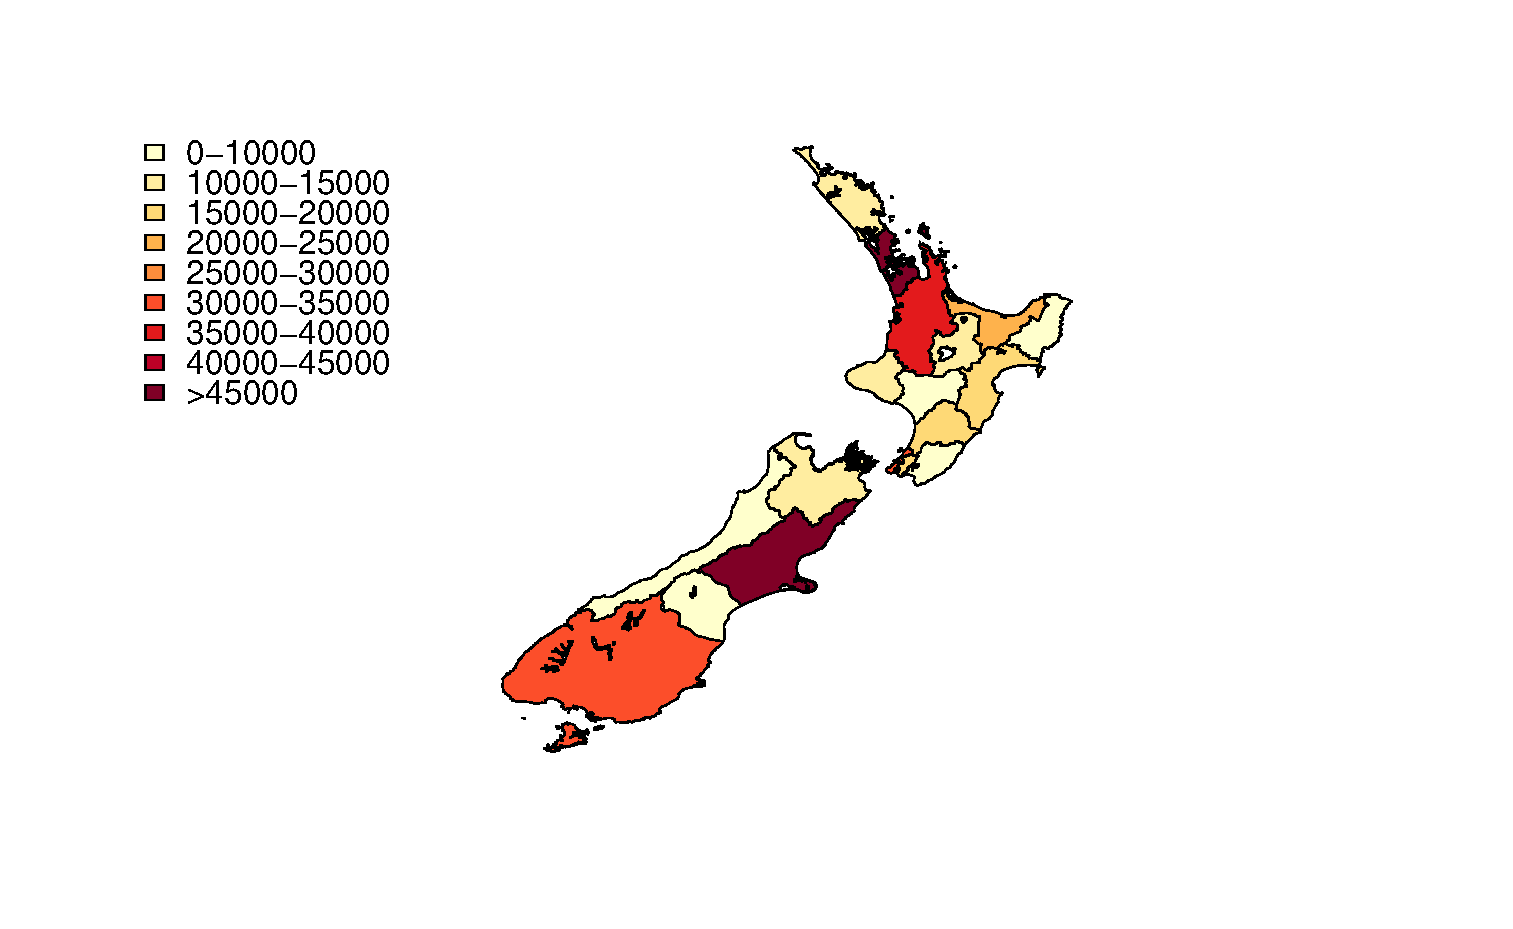
\includegraphics[width=0.9\textwidth]{naive_map.pdf}
     \end{center}
     \caption{Numbers of na\"{\i}ve individuals per District Health Board, using national immunity data (\autoref{table:sero})}
     \label{fig:naive_map}
\end{figure}

\subsection{Population immunity results}
\label{sub:popim}

 \vspace{5mm} %5mm vertical space
\begin{table}
%latex.default(t12006[1:7], file = "", table.env = FALSE, rowname = NULL)%
\begin{center}
\begin{tabular}{rrrrrrr}
\hline\hline
\multicolumn{1}{c}{Min}&\multicolumn{1}{c}{1st Q}&\multicolumn{1}{c}{Median}&\multicolumn{1}{c}{Mean}&\multicolumn{1}{c}{3rd Q}&\multicolumn{1}{c}{Max}&\multicolumn{1}{c}{NA}\tabularnewline
\hline
$0$&$0.9231$&$0.9604$&$0.9457$&$1$&$1$&$318$\tabularnewline
\hline
\end{tabular}\end{center}\caption{Summary of the proportion of 2006 birth cohort vaccinated against MMR1 across the 2013 area units. See \autoref{fig:fig12006}.}
\label{table:tab12006}
\end{table}

\begin{sidewaysfigure}
   \begin{center}
    \includegraphics[width=0.9\textwidth]{nir_census_MMR1_NIR_2006.pdf}
    \end{center}
    \caption{Proportion of the New Zealand population born in 2006 vaccinated against measles using MMR1 in each 2013 area unit. Note no adjustment is made for vaccine efficacy. The histogram shows the frequency of the proportion vaccinated across the country's area units with 95\% shown in red and the median for the cohort shown in orange. See \autoref{table:tab12006} and the supplementary data for details.}
%\end{center}
\label{fig:fig12006}
\end{sidewaysfigure}

 \vspace{5mm} %5mm vertical space
\begin{table}
%latex.default(t22006[1:7], file = "", table.env = FALSE, rowname = NULL)%
\begin{center}
\begin{tabular}{rrrrrrr}
\hline\hline
\multicolumn{1}{c}{Min}&\multicolumn{1}{c}{1st Q}&\multicolumn{1}{c}{Median}&\multicolumn{1}{c}{Mean}&\multicolumn{1}{c}{3rd Q}&\multicolumn{1}{c}{Max}&\multicolumn{1}{c}{NA}\tabularnewline
\hline
$0$&$0.8611$&$0.9167$&$0.9029$&$0.9714$&$1.143$&$318$\tabularnewline
\hline
\end{tabular}\end{center}\caption{Summary of the proportion of 2006 birth cohort vaccinated against MMR2 across the 2013 area units. See \autoref{fig:fig22006}.}
\label{table:tab22006}
\end{table}


\begin{sidewaysfigure}
\begin{center}
\includegraphics[width=0.9\textwidth]{nir_census_MMR2_NIR_2006.pdf}
\end{center}
    \caption{Proportion of the New Zealand population born in 2006 vaccinated against measles using MMR2 in each 2013 area unit. Note no adjustment is made for vaccine efficacy. The histogram shows the frequency of the proportion vaccinated across the country's area units with 95\% shown in red and the median for the cohort shown in orange. See \autoref{table:tab22006} and the supplementary data for details.}
% \end{center}
\label{fig:fig22006}
\end{sidewaysfigure}

 \vspace{5mm} %5mm vertical space
\begin{table}
%latex.default(t12007[1:7], file = "", table.env = FALSE, rowname = NULL)%
\begin{center}
\begin{tabular}{rrrrrrr}
\hline\hline
\multicolumn{1}{c}{Min}&\multicolumn{1}{c}{1st Q}&\multicolumn{1}{c}{Median}&\multicolumn{1}{c}{Mean}&\multicolumn{1}{c}{3rd Q}&\multicolumn{1}{c}{Max}&\multicolumn{1}{c}{NA}\tabularnewline
\hline
$0$&$0.9286$&$0.9621$&$0.9499$&$1$&$1$&$324$\tabularnewline
\hline
\end{tabular}\end{center}\caption{Summary of the proportion of 2007 birth cohort vaccinated against MMR1 across the 2013 area units. See \autoref{fig:fig12007}.}
\label{table:tab12007}
\end{table}

\begin{sidewaysfigure}
\begin{center}
\includegraphics[width=0.9\textwidth]{nir_census_MMR1_NIR_2007.pdf}
\end{center}
    \caption{Proportion of the New Zealand population born in 2007 vaccinated against measles using MMR1 in each 2013 area unit. Note no adjustment is made for vaccine efficacy. The histogram shows the frequency of the proportion vaccinated across the country's area units with 95\% shown in red and the median for the cohort shown in orange. See \autoref{table:tab12007} and the supplementary data for details.}
% \end{center}
\label{fig:fig12007}
\end{sidewaysfigure}

 \vspace{5mm} %5mm vertical space
\begin{table}
%latex.default(t22007[1:7], file = "", table.env = FALSE, rowname = NULL)%
\begin{center}
\begin{tabular}{rrrrrrr}
\hline\hline
\multicolumn{1}{c}{Min}&\multicolumn{1}{c}{1st Q}&\multicolumn{1}{c}{Median}&\multicolumn{1}{c}{Mean}&\multicolumn{1}{c}{3rd Q}&\multicolumn{1}{c}{Max}&\multicolumn{1}{c}{NA}\tabularnewline
\hline
$0$&$0.8592$&$0.9099$&$0.899$&$0.9643$&$1$&$324$\tabularnewline
\hline
\end{tabular}\end{center}\caption{Summary of the proportion of 2007 birth cohort vaccinated against MMR2 across the 2013 area units. See \autoref{fig:fig22007}.}
\label{table:tab22007}
\end{table}

\begin{sidewaysfigure}
\begin{center}
    \includegraphics[width=0.9\textwidth]{nir_census_MMR2_NIR_2007.pdf}
\end{center}
    \caption{Proportion of the New Zealand population born in 2007 vaccinated against measles using MMR2 in each 2013 area unit. Note no adjustment is made for vaccine efficacy. The histogram shows the frequency of the proportion vaccinated across the country's area units with 95\% shown in red and the median for the cohort shown in orange. See \autoref{table:tab22007} and the supplementary data for details.}
% \end{center}
\label{fig:fig22007}
\end{sidewaysfigure}

 \vspace{5mm} %5mm vertical space
\begin{table}
%latex.default(t12008[1:7], file = "", table.env = FALSE, rowname = NULL)%
\begin{center}
\begin{tabular}{rrrrrrr}
\hline\hline
\multicolumn{1}{c}{Min}&\multicolumn{1}{c}{1st Q}&\multicolumn{1}{c}{Median}&\multicolumn{1}{c}{Mean}&\multicolumn{1}{c}{3rd Q}&\multicolumn{1}{c}{Max}&\multicolumn{1}{c}{NA}\tabularnewline
\hline
$0$&$0.9365$&$0.971$&$0.9569$&$1$&$1$&$315$\tabularnewline
\hline
\end{tabular}\end{center}\caption{Summary of the proportion of 2008 birth cohort vaccinated against MMR1 across the 2013 area units. See \autoref{fig:fig12008}.}
\label{table:tab12008}
\end{table}

\begin{sidewaysfigure}
\begin{center}
    \includegraphics[width=0.9\textwidth]{nir_census_MMR1_NIR_2008.pdf}
\end{center}
    \caption{Proportion of the New Zealand population born in 2008 vaccinated against measles using MMR1 in each 2013 area unit. Note no adjustment is made for vaccine efficacy. The histogram shows the frequency of the proportion vaccinated across the country's area units with 95\% shown in red and the median for the cohort shown in orange. See \autoref{table:tab12008} and the supplementary data for details.}
% \end{center}
\label{fig:fig12008}
\end{sidewaysfigure}

 \vspace{5mm} %5mm vertical space
\begin{table}
%latex.default(t22008[1:7], file = "", table.env = FALSE, rowname = NULL)%
\begin{center}
\begin{tabular}{rrrrrrr}
\hline\hline
\multicolumn{1}{c}{Min}&\multicolumn{1}{c}{1st Q}&\multicolumn{1}{c}{Median}&\multicolumn{1}{c}{Mean}&\multicolumn{1}{c}{3rd Q}&\multicolumn{1}{c}{Max}&\multicolumn{1}{c}{NA}\tabularnewline
\hline
$0$&$0.8451$&$0.9048$&$0.8908$&$0.9583$&$1$&$315$\tabularnewline
\hline
\end{tabular}\end{center}\caption{Summary of the proportion of 2008 birth cohort vaccinated against MMR2 across the 2013 area units. See \autoref{fig:fig22008}.}
\label{table:tab22008}
\end{table}

\begin{sidewaysfigure}
\begin{center}
    \includegraphics[width=0.9\textwidth]{nir_census_MMR2_NIR_2008.pdf}
 \end{center}
    \caption{Proportion of the New Zealand population born in 2008 vaccinated against measles using MMR2 in each 2013 area unit. Note no adjustment is made for vaccine efficacy. The histogram shows the frequency of the proportion vaccinated across the country's area units with 95\% shown in red and the median for the cohort shown in orange. See \autoref{table:tab22008} and the supplementary data for details.}
% \end{center}
\label{fig:fig22008}
\end{sidewaysfigure}

 \vspace{5mm} %5mm vertical space
\begin{table}
%latex.default(t12009[1:7], file = "", table.env = FALSE, rowname = NULL)%
\begin{center}
\begin{tabular}{rrrrrrr}
\hline\hline
\multicolumn{1}{c}{Min}&\multicolumn{1}{c}{1st Q}&\multicolumn{1}{c}{Median}&\multicolumn{1}{c}{Mean}&\multicolumn{1}{c}{3rd Q}&\multicolumn{1}{c}{Max}&\multicolumn{1}{c}{NA}\tabularnewline
\hline
$0$&$0.939$&$0.9722$&$0.9575$&$1$&$1$&$324$\tabularnewline
\hline
\end{tabular}\end{center}\caption{Summary of the proportion of 2009 birth cohort vaccinated against MMR1 across the 2013 area units. See \autoref{fig:fig12009}.}
\label{table:tab12009}
\end{table}

\begin{sidewaysfigure}
\begin{center}
    \includegraphics[width=0.9\textwidth]{nir_census_MMR1_NIR_2009.pdf}
 \end{center}
    \caption{Proportion of the New Zealand population born in 2009 vaccinated against measles using MMR1 in each 2013 area unit. Note no adjustment is made for vaccine efficacy. The histogram shows the frequency of the proportion vaccinated across the country's area units with 95\% shown in red and the median for the cohort shown in orange. See \autoref{table:tab12009} and the supplementary data for details.}
%\end{center}
\label{fig:fig12009}
\end{sidewaysfigure}

 \vspace{5mm} %5mm vertical space
\begin{table}
%latex.default(t22009[1:7], file = "", table.env = FALSE, rowname = NULL)%
\begin{center}
\begin{tabular}{rrrrrrr}
\hline\hline
\multicolumn{1}{c}{Min}&\multicolumn{1}{c}{1st Q}&\multicolumn{1}{c}{Median}&\multicolumn{1}{c}{Mean}&\multicolumn{1}{c}{3rd Q}&\multicolumn{1}{c}{Max}&\multicolumn{1}{c}{NA}\tabularnewline
\hline
$0$&$0.8302$&$0.8889$&$0.8773$&$0.9444$&$1$&$324$\tabularnewline
\hline
\end{tabular}\end{center}\caption{Summary of the proportion of 2009 birth cohort vaccinated against MMR2 across the 2013 area units. See \autoref{fig:fig22009}.}
\label{table:tab22009}
\end{table}

\begin{sidewaysfigure}
\begin{center}
    \includegraphics[width=0.9\textwidth]{nir_census_MMR2_NIR_2009.pdf}
 \end{center}
    \caption{Proportion of the New Zealand population born in 2009 vaccinated against measles using MMR2 in each 2013 area unit. Note no adjustment is made for vaccine efficacy. The histogram shows the frequency of the proportion vaccinated across the country's area units with 95\% shown in red and the median for the cohort shown in orange. See \autoref{table:tab22009} and the supplementary data for details.}
%\end{center}
\label{fig:fig22009}
\end{sidewaysfigure}

 \vspace{5mm} %5mm vertical space
\begin{table}
%latex.default(t12010[1:7], file = "", table.env = FALSE, rowname = NULL)%
\begin{center}
\begin{tabular}{rrrrrrr}
\hline\hline
\multicolumn{1}{c}{Min}&\multicolumn{1}{c}{1st Q}&\multicolumn{1}{c}{Median}&\multicolumn{1}{c}{Mean}&\multicolumn{1}{c}{3rd Q}&\multicolumn{1}{c}{Max}&\multicolumn{1}{c}{NA}\tabularnewline
\hline
$0.0714$&$0.9326$&$0.9667$&$0.9557$&$1$&$1$&$321$\tabularnewline
\hline
\end{tabular}\end{center}\caption{Summary of the proportion of 2010 birth cohort vaccinated against MMR1 across the 2013 area units. See \autoref{fig:fig12010}.}
\label{table:tab12010}
\end{table}

\begin{sidewaysfigure}
\begin{center}
    \includegraphics[width=0.9\textwidth]{nir_census_MMR1_NIR_2010.pdf}
\end{center}
    \caption{Proportion of the New Zealand population born in 2010 vaccinated against measles using MMR1 in each 2013 area unit. Note no adjustment is made for vaccine efficacy. The histogram shows the frequency of the proportion vaccinated across the country's area units with 95\% shown in red and the median for the cohort shown in orange. See \autoref{table:tab12010} and the supplementary data for details.}
%\end{center}
\label{fig:fig12010}
\end{sidewaysfigure}

 \vspace{5mm} %5mm vertical space
\begin{table}
%latex.default(t22010[1:7], file = "", table.env = FALSE, rowname = NULL)%
\begin{center}
\begin{tabular}{rrrrrrr}
\hline\hline
\multicolumn{1}{c}{Min}&\multicolumn{1}{c}{1st Q}&\multicolumn{1}{c}{Median}&\multicolumn{1}{c}{Mean}&\multicolumn{1}{c}{3rd Q}&\multicolumn{1}{c}{Max}&\multicolumn{1}{c}{NA}\tabularnewline
\hline
$0$&$0.625$&$0.7059$&$0.6974$&$0.7791$&$1$&$321$\tabularnewline
\hline
\end{tabular}\end{center}\caption{Summary of the proportion of 2010 birth cohort vaccinated against MMR2 across the 2013 area units. See \autoref{fig:fig22010}.}
\label{table:tab22010}
\end{table}

\begin{sidewaysfigure}
\begin{center}
    \includegraphics[width=0.9\textwidth]{nir_census_MMR2_NIR_2010.pdf}
 \end{center}
    \caption{Proportion of the New Zealand population born in 2010 vaccinated against measles using MMR2 in each 2013 area unit. Note no adjustment is made for vaccine efficacy. The histogram shows the frequency of the proportion vaccinated across the country's area units with 95\% shown in red and the median for the cohort shown in orange. See \autoref{table:tab22010} and the supplementary data for details.}
%\end{center}
\label{fig:fig22010}
\end{sidewaysfigure}

 \vspace{5mm} %5mm vertical space
\begin{table}
%latex.default(t12011[1:7], file = "", table.env = FALSE, rowname = NULL)%
\begin{center}
\begin{tabular}{rrrrrrr}
\hline\hline
\multicolumn{1}{c}{Min}&\multicolumn{1}{c}{1st Q}&\multicolumn{1}{c}{Median}&\multicolumn{1}{c}{Mean}&\multicolumn{1}{c}{3rd Q}&\multicolumn{1}{c}{Max}&\multicolumn{1}{c}{NA}\tabularnewline
\hline
$0$&$0.9286$&$0.9643$&$0.9492$&$1$&$1$&$326$\tabularnewline
\hline
\end{tabular}\end{center}\caption{Summary of the proportion of 2011 birth cohort vaccinated against MMR1 across the 2013 area units. See \autoref{fig:fig12011}.}
\label{table:tab12011}
\end{table}

\begin{sidewaysfigure}
\begin{center}
    \includegraphics[width=0.9\textwidth]{nir_census_MMR1_NIR_2011.pdf}
 \end{center}
    \caption{Proportion of the New Zealand population born in 2011 vaccinated against measles using MMR1 in each 2013 area unit. Note no adjustment is made for vaccine efficacy. The histogram shows the frequency of the proportion vaccinated across the country's area units with 95\% shown in red and the median for the cohort shown in orange. See \autoref{table:tab12011} and the supplementary data for details.}
%\end{center}
\label{fig:fig12011}
\end{sidewaysfigure}

 \vspace{5mm} %5mm vertical space
\begin{table}
%latex.default(t22011[1:7], file = "", table.env = FALSE, rowname = NULL)%
\begin{center}
\begin{tabular}{rrrrrrr}
\hline\hline
\multicolumn{1}{c}{Min}&\multicolumn{1}{c}{1st Q}&\multicolumn{1}{c}{Median}&\multicolumn{1}{c}{Mean}&\multicolumn{1}{c}{3rd Q}&\multicolumn{1}{c}{Max}&\multicolumn{1}{c}{NA}\tabularnewline
\hline
$0$&$0$&$0.0345$&$0.0606$&$0.0893$&$1$&$326$\tabularnewline
\hline
\end{tabular}\end{center}\caption{Summary of the proportion of 2011 birth cohort vaccinated against MMR2 across the 2013 area units. See \autoref{fig:fig22011}.}
\label{table:tab22011}
\end{table}

\begin{sidewaysfigure}
\begin{center}
    \includegraphics[width=0.9\textwidth]{nir_census_MMR2_NIR_2011.pdf}
 \end{center}
    \caption{Proportion of the New Zealand population born in 2011 vaccinated against measles using MMR2 in each 2013 area unit. Note no adjustment is made for vaccine efficacy. The histogram shows the frequency of the proportion vaccinated across the country's area units with 95\% shown in red and the median for the cohort shown in orange. See \autoref{table:tab22011} and the supplementary data for details.}
%\end{center}
\label{fig:fig22011}
\end{sidewaysfigure}

 \vspace{5mm} %5mm vertical space
\begin{table}
%latex.default(t12012[1:7], file = "", table.env = FALSE, rowname = NULL)%
\begin{center}
\begin{tabular}{rrrrrrr}
\hline\hline
\multicolumn{1}{c}{Min}&\multicolumn{1}{c}{1st Q}&\multicolumn{1}{c}{Median}&\multicolumn{1}{c}{Mean}&\multicolumn{1}{c}{3rd Q}&\multicolumn{1}{c}{Max}&\multicolumn{1}{c}{NA}\tabularnewline
\hline
$0$&$0.9333$&$0.9667$&$0.9527$&$1$&$1$&$331$\tabularnewline
\hline
\end{tabular}\end{center}\caption{Summary of the proportion of 2012 birth cohort vaccinated against MMR1 across the 2013 area units. See \autoref{fig:fig12012}.}
\label{table:tab12012}
\end{table}

\begin{sidewaysfigure}
\begin{center}
    \includegraphics[width=0.9\textwidth]{nir_census_MMR1_NIR_2012.pdf}
 \end{center}
    \caption{Proportion of the New Zealand population born in 2012 vaccinated against measles using MMR1 in each 2013 area unit. Note no adjustment is made for vaccine efficacy. The histogram shows the frequency of the proportion vaccinated across the country's area units with 95\% shown in red and the median for the cohort shown in orange. See \autoref{table:tab12012} and the supplementary data for details.}
%\end{center}
\label{fig:fig12012}
\end{sidewaysfigure}

 \vspace{5mm} %5mm vertical space
\begin{table}
%latex.default(t22012[1:7], file = "", table.env = FALSE, rowname = NULL)%
\begin{center}
\begin{tabular}{rrrrrrr}
\hline\hline
\multicolumn{1}{c}{Min}&\multicolumn{1}{c}{1st Q}&\multicolumn{1}{c}{Median}&\multicolumn{1}{c}{Mean}&\multicolumn{1}{c}{3rd Q}&\multicolumn{1}{c}{Max}&\multicolumn{1}{c}{NA}\tabularnewline
\hline
$0$&$0$&$0.0041$&$0.0403$&$0.0476$&$1$&$331$\tabularnewline
\hline
\end{tabular}\end{center}\caption{Summary of the proportion of 2012 birth cohort vaccinated against MMR2 across the 2013 area units. See \autoref{fig:fig22012}.}
\label{table:tab22012}
\end{table}

\begin{sidewaysfigure}
\begin{center}
    \includegraphics[width=0.9\textwidth]{nir_census_MMR2_NIR_2012.pdf}
 \end{center}
    \caption{Proportion of the New Zealand population born in 2012 vaccinated against measles using MMR2 in each 2013 area unit. Note no adjustment is made for vaccine efficacy. The histogram shows the frequency of the proportion vaccinated across the country's area units with 95\% shown in red and the median for the cohort shown in orange. See \autoref{table:tab22012} and the supplementary data for details.}
% \end{center}
\label{fig:fig22012}
\end{sidewaysfigure}

 \vspace{5mm} %5mm vertical space
\begin{table}
%latex.default(t12013[1:7], file = "", table.env = FALSE, rowname = NULL)%
\begin{center}
\begin{tabular}{rrrrrrr}
\hline\hline
\multicolumn{1}{c}{Min}&\multicolumn{1}{c}{1st Q}&\multicolumn{1}{c}{Median}&\multicolumn{1}{c}{Mean}&\multicolumn{1}{c}{3rd Q}&\multicolumn{1}{c}{Max}&\multicolumn{1}{c}{NA}\tabularnewline
\hline
$0$&$0.5556$&$0.6333$&$0.6276$&$0.7$&$1$&$331$\tabularnewline
\hline
\end{tabular}\end{center}\caption{Summary of the proportion of 2006 birth cohort vaccinated against MMR1 across the 2013 area units. See \autoref{fig:fig12013}.}
\label{table:tab12013}
\end{table}

\begin{sidewaysfigure}
\begin{center}
    \includegraphics[width=0.9\textwidth]{nir_census_MMR1_NIR_2013.pdf}
 \end{center}
    \caption{Proportion of the New Zealand population born in 2013 vaccinated against measles using MMR1 in each 2013 area unit. Note no adjustment is made for vaccine efficacy. The histogram shows the frequency of the proportion vaccinated across the country's area units with 95\% shown in red and the median for the cohort shown in orange. See \autoref{table:tab12013} and the supplementary data for details.}
% \end{center}
\label{fig:fig12013}
\end{sidewaysfigure}

 \vspace{5mm} %5mm vertical space
\begin{table}
%latex.default(t22013[1:7], file = "", table.env = FALSE, rowname = NULL)%
\begin{center}
\begin{tabular}{rrrrrrr}
\hline\hline
\multicolumn{1}{c}{Min}&\multicolumn{1}{c}{1st Q}&\multicolumn{1}{c}{Median}&\multicolumn{1}{c}{Mean}&\multicolumn{1}{c}{3rd Q}&\multicolumn{1}{c}{Max}&\multicolumn{1}{c}{NA}\tabularnewline
\hline
$0$&$0$&$0$&$0.0217$&$0.0263$&$1$&$331$\tabularnewline
\hline
\end{tabular}\end{center}\caption{Summary of the proportion of 2006 birth cohort vaccinated against MMR2 across the 2013 area units. See \autoref{fig:fig22013}.}
\label{table:tab22013}
\end{table}

\begin{sidewaysfigure}
\begin{center}
    \includegraphics[width=0.9\textwidth]{nir_census_MMR2_NIR_2013.pdf}
\end{center}
\caption{Proportion of the New Zealand population born in 2013 vaccinated against measles using MMR2 in each 2013 area unit. Note no adjustment is made for vaccine efficacy. The histogram shows the frequency of the proportion vaccinated across the country's area units with 95\% shown in red and the median for the cohort shown in orange. See \autoref{table:tab22013} and the supplementary data for details.}
%     \end{center}
\label{fig:fig22013}
\end{sidewaysfigure}

 \vspace{5mm} %5mm vertical space
\begin{table}
%latex.default(t12014[1:7], file = "", table.env = FALSE, rowname = NULL)%
\begin{center}
\begin{tabular}{rrrrrrr}
\hline\hline
\multicolumn{1}{c}{Min}&\multicolumn{1}{c}{1st Q}&\multicolumn{1}{c}{Median}&\multicolumn{1}{c}{Mean}&\multicolumn{1}{c}{3rd Q}&\multicolumn{1}{c}{Max}&\multicolumn{1}{c}{NA}\tabularnewline
\hline
$0$&$0$&$0$&$0.0088$&$0$&$1$&$334$\tabularnewline
\hline
\end{tabular}\end{center}\caption{Summary of the proportion of 2014 birth cohort vaccinated against MMR1 across the 2013 area units. See \autoref{fig:fig12014}.}
\label{table:tab12014}
\end{table}

\begin{sidewaysfigure}
\begin{center}
    \includegraphics[width=0.9\textwidth]{nir_census_MMR1_NIR_2014.pdf}
 \end{center}
    \caption{Proportion of the New Zealand population born in 2014 vaccinated against measles using MMR1 in each 2013 area unit. Note no adjustment is made for vaccine efficacy. The histogram shows the frequency of the proportion vaccinated across the country's area units with 95\% shown in red and the median for the cohort shown in orange. See \autoref{table:tab12014} and the supplementary data for details.}
% \end{center}
\label{fig:fig12014}
\end{sidewaysfigure}

 \vspace{5mm} %5mm vertical space
\begin{table}
%latex.default(t22014[1:7], file = "", table.env = FALSE, rowname = NULL)%
\begin{center}
\begin{tabular}{rrrrrrr}
\hline\hline
\multicolumn{1}{c}{Min}&\multicolumn{1}{c}{1st Q}&\multicolumn{1}{c}{Median}&\multicolumn{1}{c}{Mean}&\multicolumn{1}{c}{3rd Q}&\multicolumn{1}{c}{Max}&\multicolumn{1}{c}{NA}\tabularnewline
\hline
$0$&$0$&$0$&$0.0067$&$0$&$1$&$334$\tabularnewline
\hline
\end{tabular}\end{center}\caption{Summary of the proportion of 2014 birth cohort vaccinated against MMR2 across the 2013 area units. See \autoref{fig:fig22014}.}
\label{table:tab22014}
\end{table}

\begin{sidewaysfigure}
\begin{center}
    \includegraphics[width=0.9\textwidth]{nir_census_MMR2_NIR_2014.pdf}
 \end{center}
\caption{Proportion of the New Zealand population born in 2014 vaccinated against measles using MMR2 in each 2013 area unit. Note no adjustment is made for vaccine efficacy. The histogram shows the frequency of the proportion vaccinated across the country's area units with 95\% shown in red and the median for the cohort shown in orange. See \autoref{table:tab22014} and the supplementary data for details.}
% \end{center}
\label{fig:fig22014}
\end{sidewaysfigure}

The majority of the na\"{\i}ve among the general New Zealand population are in their first years of life (\autoref{fig:naive}). However, the distribution of na\"{\i}ve at a national level shows that the recent MMR vaccination schemes are reducing the proportions of na\"{\i}ve population in the 3--5 year old age group to greater levels than in older young people  (\autoref{fig:naive}). Plotting the breakdown of these figures by DHB clearly shows that the greatest numbers of na\"{\i}ve people are in DHBs with larger urban areas (\autoref{fig:naive_map}). The distribution of the numbers of na\"{\i}ve and the total na\"{\i}ve populations per DHB, assuming national immunisation and immunity rates are representative, are given in the following figures in the appendix (\autoref{sec:app}): 
\begin{itemize}[noitemsep,nolistsep]
\item Northland: \autoref{fig:Northland}
\item Waitemata: \autoref{fig:Waitemata}
\item Auckland: \autoref{fig:Auckland}
\item Counties Manukau: \autoref{fig:Counties_Manukau}
\item Waikato: \autoref{fig:Waikato}
\item Lakes: \autoref{fig:Lakes}
\item Bay of Plenty: \autoref{fig:BayofPlenty}
\item Tairawhiti: \autoref{fig:Tairawhiti}
\item Taranaki: \autoref{fig:Taranaki}
\item Hawke's Bay: \autoref{fig:HawkesBay}
\item Whanganui: \autoref{fig:Whanganui}
\item Mid-Central: \autoref{fig:Midcentral}
\item Hutt: \autoref{fig:Hutt}
\item Capital and Coast: \autoref{fig:CapitalandCoast}
\item Wairarapa: \autoref{fig:Wairarapa}
\item Nelson Marlborough: \autoref{fig:NelsonMarlborough}
\item West Coast: \autoref{fig:WestCoast}
\item Canterbury: \autoref{fig:Canterbury}
\item South Canterbury: \autoref{fig:SouthCanterbury}
\item Southern: \autoref{fig:Southern}
\end{itemize}

Plotting the lower level data available from the NIR database highlights the issue of surveillance data requiring appropriate denominator data, as these analyses show that there is a lack of correspondence between the national census data and the NIR data (\autoref{fig:naive_au}, \autoref{fig:naive_au_prop})

\subsection{Measles importation risk methods}
\label{sub:imp_risk}
For our measles importation risk analyses, we use arrivals data from New Zealand immigration and New Zealander travel destination data by country and year (\href{http://www.immigration.govt.nz/}{www.immigration.govt.nz}), to measure human movement to and from New Zealand. We collated country population size, measles incidence and measles vaccination cover from the WHO (\href{http://www.who.int/research/en/}{www.who.int/research/en/}). WHO measles coverage is the percent of children that receive one dose of measles vaccine by their second birthday. Note the immigration figures use all immigration of foreign nationals, coming for whatever purpose, and includes non-New Zealanders resident in New Zealand, but not yet holders of New Zealand passports. We use the WHO data to determine per capita measles cases for each year and use these data and the number of immigrants to New Zealand to begin to understand where measles is likely to be imported from. We use simple per capita rates for measles and the number of travellers to each country to score and map the risk of mealses importation. We use 0--19 year old data for the immigration figures, as no further details were available and it was determined this was more appropriate than using all age classes because > 19 year olds are believe to be immune to measles more or less globally. These age category data were not available for New Zealand travellers, so we use all data on all travellers. We present the data from 2013 because this year was the most recent with the relatively complete WHO measles data, and thus accounts for improved measles vaccination coverage following the United Nations Millenium Development Goals' improvements in measles vaccination coverage. Data for 2013 are less complete than 2012, but substantially better than 2014.

\subsection{Measles importation risk results}

\begin{table}
%latex.default(incidence, file = "", table.env = FALSE, rowname = NULL)%
\begin{center}
\begin{tabular}{lr}
\hline\hline
\multicolumn{1}{c}{country}&\multicolumn{1}{c}{incidence}\tabularnewline
\hline
Georgia&$1806$\tabularnewline
Namibia&$ 455$\tabularnewline
Equatorial Guinea&$ 436$\tabularnewline
Angola&$ 409$\tabularnewline
Lebanon&$ 379$\tabularnewline
Nigeria&$ 313$\tabularnewline
Somalia&$ 311$\tabularnewline
Sudan&$ 260$\tabularnewline
Lesotho&$ 251$\tabularnewline
Uganda&$ 217$\tabularnewline
Netherlands&$ 159$\tabularnewline
Central African Republic&$ 132$\tabularnewline
Turkey&$ 100$\tabularnewline
Sri Lanka&$ 100$\tabularnewline
Togo&$  85$\tabularnewline
Sudan&$  76$\tabularnewline
Gabon&$  75$\tabularnewline
Niger&$  71$\tabularnewline
Nepal&$  68$\tabularnewline
Benin&$  63$\tabularnewline
Ethiopia&$  57$\tabularnewline
Romania&$  51$\tabularnewline
Pakistan&$  49$\tabularnewline
Thailand&$  40$\tabularnewline
Indonesia&$  39$\tabularnewline
Qatar&$  36$\tabularnewline
Cameroon&$  35$\tabularnewline
Syrian Arab Republic&$  34$\tabularnewline
Djibouti&$  33$\tabularnewline
United Kingdom&$  31$\tabularnewline
\hline
\end{tabular}\end{center}\caption{Highest measles incidence per million (2013)}
\label{table:incidence12}
\end{table}

\begin{table}
%latex.default(vaccinecover, file = "", table.env = FALSE, rowname = NULL)%
\begin{center}
\begin{tabular}{lr}
\hline\hline
\multicolumn{1}{c}{country}&\multicolumn{1}{c}{cover}\tabularnewline
\hline
Central African Republic&$29$\tabularnewline
Somalia&$29$\tabularnewline
Equatorial Guinea&$41$\tabularnewline
South Sudan&$55$\tabularnewline
Lesotho&$61$\tabularnewline
Pakistan&$61$\tabularnewline
Vanuatu&$65$\tabularnewline
Gabon&$70$\tabularnewline
Marshall Islands&$70$\tabularnewline
Papua New Guinea&$70$\tabularnewline
Timor-Leste&$70$\tabularnewline
Mali&$72$\tabularnewline
Togo&$72$\tabularnewline
Nigeria&$73$\tabularnewline
Liberia&$74$\tabularnewline
San Marino&$74$\tabularnewline
Eritrea&$75$\tabularnewline
Paraguay&$75$\tabularnewline
Solomon Islands&$76$\tabularnewline
Iraq&$77$\tabularnewline
Ethiopia&$78$\tabularnewline
Haiti&$78$\tabularnewline
Yemen&$78$\tabularnewline
Chad&$79$\tabularnewline
Kenya&$79$\tabularnewline
Congo&$80$\tabularnewline
Djibouti&$80$\tabularnewline
Mauritania&$80$\tabularnewline
Zambia&$80$\tabularnewline
Afghanistan&$82$\tabularnewline
\hline
\end{tabular}\end{center}\caption{Lowest national measles vaccine cover (\%), 2013}
\label{table:cover12}
\end{table}

\begin{table}
%latex.default(im, file = "", table.env = FALSE, rowname = NULL)%
\begin{center}
\begin{tabular}{lr}
\hline\hline
\multicolumn{1}{c}{country}&\multicolumn{1}{c}{immigration}\tabularnewline
\hline
Australia&$130703$\tabularnewline
China&$ 26380$\tabularnewline
United Kingdom&$ 25155$\tabularnewline
Japan&$ 20534$\tabularnewline
United States&$ 20247$\tabularnewline
Germany&$ 14793$\tabularnewline
France&$ 12173$\tabularnewline
Korea, Republic of&$ 10398$\tabularnewline
India&$  7013$\tabularnewline
Fiji&$  6040$\tabularnewline
Malaysia&$  5981$\tabularnewline
Thailand&$  5233$\tabularnewline
Canada&$  5013$\tabularnewline
Singapore&$  4887$\tabularnewline
Samoa&$  4047$\tabularnewline
South Africa&$  3763$\tabularnewline
Tonga&$  3477$\tabularnewline
Hong Kong&$  3281$\tabularnewline
Philippines&$  3147$\tabularnewline
Taiwan&$  2915$\tabularnewline
Indonesia&$  2580$\tabularnewline
Netherlands&$  2509$\tabularnewline
Brazil&$  2265$\tabularnewline
Sweden&$  1862$\tabularnewline
Denmark&$  1605$\tabularnewline
Switzerland&$  1376$\tabularnewline
Ireland&$  1331$\tabularnewline
Chile&$  1157$\tabularnewline
Saudi Arabia&$  1141$\tabularnewline
Russia&$  1068$\tabularnewline
\hline
\end{tabular}\end{center}\caption{Non-New Zealander travel and immigration numbers, 0--19 year olds, 2013}
\label{table:imtravel12}
\end{table}

\begin{table}
%latex.default(nz, file = "", table.env = FALSE, rowname = NULL)%
\begin{center}
\begin{tabular}{lr}
\hline\hline
\multicolumn{1}{c}{country}&\multicolumn{1}{c}{immigration}\tabularnewline
\hline
Australia&$1017540$\tabularnewline
United States&$ 142200$\tabularnewline
Fiji&$ 112260$\tabularnewline
United Kingdom&$  96680$\tabularnewline
China&$  73340$\tabularnewline
Cook Islands&$  72820$\tabularnewline
Samoa&$  44060$\tabularnewline
Thailand&$  42060$\tabularnewline
India&$  40760$\tabularnewline
Indonesia&$  25100$\tabularnewline
Japan&$  21840$\tabularnewline
Canada&$  21720$\tabularnewline
Tonga&$  20120$\tabularnewline
Singapore&$  18300$\tabularnewline
Hong Kong&$  18000$\tabularnewline
Malaysia&$  17480$\tabularnewline
Philippines&$  17260$\tabularnewline
France&$  15980$\tabularnewline
Vanuatu&$  15580$\tabularnewline
South Africa&$  14000$\tabularnewline
Korea, Republic of&$  13980$\tabularnewline
Italy&$  13620$\tabularnewline
Germany&$  12800$\tabularnewline
Viet Nam&$  12640$\tabularnewline
Taiwan&$  10300$\tabularnewline
New Caledonia&$   7620$\tabularnewline
Spain&$   6560$\tabularnewline
Netherlands&$   6260$\tabularnewline
Papua New Guinea&$   6200$\tabularnewline
Ireland&$   6160$\tabularnewline
\hline
\end{tabular}\end{center}\caption{New Zealander travel numbers by destination, 2013}
\label{table:nztravel12}
\end{table}

\begin{table}
%latex.default(immigration, file = "", table.env = FALSE, rowname = NULL)%
\begin{center}
\begin{tabular}{lr}
\hline\hline
\multicolumn{1}{c}{country}&\multicolumn{1}{c}{immigration}\tabularnewline
\hline
Australia&$1148243$\tabularnewline
United States&$ 162447$\tabularnewline
United Kingdom&$ 121835$\tabularnewline
Fiji&$ 118300$\tabularnewline
China&$  99720$\tabularnewline
Samoa&$  48107$\tabularnewline
India&$  47773$\tabularnewline
Thailand&$  47293$\tabularnewline
Japan&$  42374$\tabularnewline
France&$  28153$\tabularnewline
Indonesia&$  27680$\tabularnewline
Germany&$  27593$\tabularnewline
Canada&$  26733$\tabularnewline
Korea, Republic of&$  24378$\tabularnewline
Tonga&$  23597$\tabularnewline
Malaysia&$  23461$\tabularnewline
Singapore&$  23187$\tabularnewline
Hong Kong&$  21281$\tabularnewline
Philippines&$  20407$\tabularnewline
South Africa&$  17763$\tabularnewline
Vanuatu&$  15748$\tabularnewline
Italy&$  14617$\tabularnewline
Viet Nam&$  13680$\tabularnewline
Taiwan&$  13215$\tabularnewline
Netherlands&$   8769$\tabularnewline
Ireland&$   7491$\tabularnewline
Spain&$   7118$\tabularnewline
Papua New Guinea&$   6457$\tabularnewline
Sri Lanka&$   5764$\tabularnewline
Brazil&$   5245$\tabularnewline
\hline
\end{tabular}\end{center}\caption{Total New Zealand traveller numbers by country (New Zealand nationals and 0--19 year old immigrants, 2013)}
\label{table:immigration12}
\end{table}

\begin{table}
%latex.default(risk, file = "", table.env = FALSE, rowname = NULL)%
\begin{center}
\begin{tabular}{lr}
\hline\hline
\multicolumn{1}{c}{country}&\multicolumn{1}{c}{risk}\tabularnewline
\hline
Australia&$7870820$\tabularnewline
United Kingdom&$3723960$\tabularnewline
China&$1928613$\tabularnewline
Thailand&$1870193$\tabularnewline
Netherlands&$1391896$\tabularnewline
Indonesia&$1071788$\tabularnewline
Philippines&$ 616175$\tabularnewline
Germany&$ 590184$\tabularnewline
Sri Lanka&$ 575635$\tabularnewline
India&$ 532515$\tabularnewline
Turkey&$ 350451$\tabularnewline
Viet Nam&$ 169200$\tabularnewline
Malaysia&$ 156460$\tabularnewline
Namibia&$ 151083$\tabularnewline
Nepal&$ 134525$\tabularnewline
France&$ 119768$\tabularnewline
Switzerland&$ 109766$\tabularnewline
Nigeria&$ 101638$\tabularnewline
Angola&$  98652$\tabularnewline
Japan&$  76407$\tabularnewline
Pakistan&$  73853$\tabularnewline
Uganda&$  70444$\tabularnewline
Canada&$  62923$\tabularnewline
Lebanon&$  57601$\tabularnewline
Russia&$  55743$\tabularnewline
Romania&$  34971$\tabularnewline
Ethiopia&$  21876$\tabularnewline
Sweden&$  21674$\tabularnewline
Sudan&$  21024$\tabularnewline
Spain&$  20552$\tabularnewline
\hline
\end{tabular}\end{center}\caption{Risk of measles importation to New Zealand in 2013, estimated by 0--19 year old international and all New Zealander traveller numbers multiplied by measles incidence in the source or destination location, see also \autoref{table:nzrisk12} and \autoref{table:imrisk12}}
\label{table:risk12}
\end{table}

\begin{table}
%latex.default(nzrisk, file = "", table.env = FALSE, rowname = NULL)%
\begin{center}
\begin{tabular}{lr}
\hline\hline
\multicolumn{1}{c}{country}&\multicolumn{1}{c}{risk}\tabularnewline
\hline
Australia&$6974895$\tabularnewline
United Kingdom&$2955082$\tabularnewline
Thailand&$1663255$\tabularnewline
China&$1418417$\tabularnewline
Netherlands&$ 993645$\tabularnewline
Indonesia&$ 971888$\tabularnewline
Philippines&$ 521154$\tabularnewline
Sri Lanka&$ 499336$\tabularnewline
India&$ 454343$\tabularnewline
Turkey&$ 342245$\tabularnewline
Germany&$ 273778$\tabularnewline
Viet Nam&$ 156336$\tabularnewline
Namibia&$ 145622$\tabularnewline
Nepal&$ 125990$\tabularnewline
Malaysia&$ 116573$\tabularnewline
Angola&$  98243$\tabularnewline
Nigeria&$  87565$\tabularnewline
Switzerland&$  79655$\tabularnewline
Uganda&$  69360$\tabularnewline
France&$  67982$\tabularnewline
Pakistan&$  53765$\tabularnewline
Lebanon&$  53054$\tabularnewline
Canada&$  51123$\tabularnewline
Japan&$  39381$\tabularnewline
Russia&$  38275$\tabularnewline
Georgia&$  36127$\tabularnewline
Romania&$  31378$\tabularnewline
Ethiopia&$  19471$\tabularnewline
Spain&$  18941$\tabularnewline
Qatar&$  16373$\tabularnewline
\hline
\end{tabular}\end{center}\caption{Risk of measles importation to New Zealand due to New Zealander travel in 2013, estimated by all traveller numbers multiplied by measles incidence in the source or destination location, see also \autoref{table:imrisk12} and \autoref{table:risk12}}
\label{table:nzrisk12}
\end{table}

\begin{table}
%latex.default(imrisk, file = "", table.env = FALSE, rowname = NULL)%
\begin{center}
\begin{tabular}{lr}
\hline\hline
\multicolumn{1}{c}{country}&\multicolumn{1}{c}{risk}\tabularnewline
\hline
Australia&$895925$\tabularnewline
United Kingdom&$768878$\tabularnewline
China&$510197$\tabularnewline
Netherlands&$398252$\tabularnewline
Germany&$316406$\tabularnewline
Thailand&$206938$\tabularnewline
Indonesia&$ 99899$\tabularnewline
Philippines&$ 95021$\tabularnewline
India&$ 78172$\tabularnewline
Sri Lanka&$ 76299$\tabularnewline
France&$ 51786$\tabularnewline
Malaysia&$ 39887$\tabularnewline
Japan&$ 37026$\tabularnewline
Switzerland&$ 30111$\tabularnewline
Pakistan&$ 20088$\tabularnewline
Russia&$ 17469$\tabularnewline
Nigeria&$ 14073$\tabularnewline
Viet Nam&$ 12863$\tabularnewline
Canada&$ 11799$\tabularnewline
Sweden&$  9984$\tabularnewline
Nepal&$  8535$\tabularnewline
Turkey&$  8206$\tabularnewline
Namibia&$  5461$\tabularnewline
Sudan&$  5451$\tabularnewline
Denmark&$  4874$\tabularnewline
Lebanon&$  4547$\tabularnewline
Somalia&$  4046$\tabularnewline
Romania&$  3593$\tabularnewline
Afghanistan&$  2437$\tabularnewline
Ethiopia&$  2405$\tabularnewline
\hline
\end{tabular}\end{center}\caption{Risk of measles importation to New Zealand due to non-New Zealander 0--19 year old travel and immigration in 2013, estimated by traveller numbers multiplied by measles incidence in the source or destination location, see also \autoref{table:nzrisk12} and \autoref{table:risk12}}
\label{table:imrisk12}
\end{table}

\begin{table}
%latex.default(toprisk2, file = "", table.env = FALSE, rowname = NULL)%
\begin{center}
\begin{tabular}{lrrr}
\hline\hline
\multicolumn{1}{c}{country}&\multicolumn{1}{c}{incidence}&\multicolumn{1}{c}{cover}&\multicolumn{1}{c}{immigration}\tabularnewline
\hline
Australia&$  7$&$94$&$1148243$\tabularnewline
United Kingdom&$ 31$&$95$&$ 121835$\tabularnewline
China&$ 19$&$99$&$  99720$\tabularnewline
Thailand&$ 40$&$99$&$  47293$\tabularnewline
Netherlands&$159$&$96$&$   8769$\tabularnewline
Indonesia&$ 39$&$89$&$  27680$\tabularnewline
Philippines&$ 30$&$90$&$  20407$\tabularnewline
Germany&$ 21$&$97$&$  27593$\tabularnewline
Sri Lanka&$100$&$99$&$   5764$\tabularnewline
India&$ 11$&$88$&$  47773$\tabularnewline
\hline
\end{tabular}\end{center}\caption{Measles and travel data from 2013 for the top 10 countries identified as high risk for measles importation. incidence: measles incidence per million; cover: percent vaccination cover (\% children that receive one dose of measles vaccine by their second birthday.); immigration: the number of New Zealander and 0--19 year old foreign national travellers entering New Zealand from the country}
\label{table:toprisk}
\end{table}

Globally, analyses of the most complete and recent year of data available, 2013, suggest measles incidence highest  and vaccination coverage is lowest in less developed nations (\autoref{table:incidence12} and \autoref{table:cover12}, and \autoref{fig:incidence12} and \autoref{fig:cover12}). Immigration by 0--19 year old non-New Zealanders (whether for work, pleasure, etc.) is dominated by people from Australia \autoref{table:imtravel12} and \autoref{fig:immigration12}. A number of other countries then follow, including United Kingdom, China, Japan and the United States. Travel by New Zealanders is also dominated by that to Australia (\autoref{table:nztravel12} and \autoref{fig:nztravel12}). Together, these mean that the greatest travel location for New Zealanders and immigration origin is from Australia (\autoref{table:immigration12} and \autoref{fig:immigration12}). However, many South Pacific nations also appear in the most visited country list by New Zealanders. Though the precise interactions between these different risk factors are unknown, the most simple, a product of measles incidence in 2013 and immigration numbers of 0--19 year olds in 2013, suggest that those countries with greatest international travel, Australia, UK, China and South East Asian countries, pose the greatest risk to New Zealand for measles importation. Though immigration from and travel to some Asian countries is lower, some Asian countries also poses a high risk of measles importation to New Zealand. Note the South Pacific island do not appear to pose a greater risk, despite large numbers of travellers of New Zealand origin, perhaps because of low measles incidence in these nations. These data are shown in \autoref{table:risk12}. The breakdown of risk of measles importation by New Zealander and non-New Zealander travellers is in \autoref{table:nzrisk12} and \autoref{table:imrisk12} and \autoref{fig:nzrisk12} and \autoref{fig:imrisk12}. The measles incidence and vaccination coverage for those countries identified as posing the greatest risk for measles importation to New Zealand are in \autoref{table:toprisk}. 

\begin{sidewaysfigure}
\begin{center}
     \includegraphics[width=0.9\textwidth]{2013totnp2.pdf}
\end{center}
\caption{Measles incidence per million, 2013. Data: WHO (\href{http://www.who.int/research/en/}{www.who.int/research/en/}). Grey indicates not reported.}
\label{fig:incidence12}
\end{sidewaysfigure}

\begin{sidewaysfigure}
\begin{center}
     \includegraphics[width=0.9\textwidth]{2013totnp3.pdf}
\end{center}
\caption{Measles vaccination cover (\% coverage of children that receive one dose of measles vaccine by their second birthday.), 2013. Data: WHO (\href{http://www.who.int/research/en/}{www.who.int/research/en/}). Grey indicates not reported.}
\label{fig:cover12}
\end{sidewaysfigure}

\begin{sidewaysfigure}
\begin{center}
     \includegraphics[width=0.9\textwidth]{2013np1.pdf}
\end{center}
\caption{Non-New Zealander international travel and immigration by 0--19 year olds, 2013)}
\label{fig:immigration12}
\end{sidewaysfigure}

\begin{sidewaysfigure}
\begin{center}
     \includegraphics[width=0.9\textwidth]{2013nznp1.pdf}
\end{center}
\caption{New Zealander international travel, 2013}
\label{fig:nztravel12}
\end{sidewaysfigure}

\begin{sidewaysfigure}
\begin{center}
     \includegraphics[width=0.9\textwidth]{2013totnp1.pdf}
\end{center}
\caption{Total international travel by 0--19 year old non New Zealanders and all ages of New Zealanders, 2013}
\label{fig:travel12}
\end{sidewaysfigure}

\begin{sidewaysfigure}
\begin{center}
     \includegraphics[width=0.9\textwidth]{2013totnp4.pdf}
\end{center}
\caption{Risk map for measles importation, based on measles incidence and non New Zealander 0--19 year old and all ages of New Zealander travel figures, 2013)}
\label{fig:risk12}
\end{sidewaysfigure}

\begin{sidewaysfigure}
\begin{center}
     \includegraphics[width=0.9\textwidth]{2013nznp4.pdf}
\end{center}
\caption{Risk map for measles importation from New Zealander international travel, based on measles incidence and travel figures, 2013}
\label{fig:nzrisk12}
\end{sidewaysfigure}

\begin{sidewaysfigure}
\begin{center}
     \includegraphics[width=0.9\textwidth]{2013np4.pdf}
\end{center}
\caption{Risk map for measles importation from 0--19 year old non-New Zealander international travel and immigration and measles incidence, 2013}
\label{fig:imrisk12}
\end{sidewaysfigure}

\begin{figure}
\begin{center}
\includegraphics{draftfinalreport_v3-032}
\end{center}
\caption{Trend in global per capita measles incidence}
\label{fig:trendincidence}
\end{figure}

\begin{figure}[H]
     \begin{center}
     \includegraphics[width=0.9\textwidth]{nzers.pdf}
     \end{center}
     \caption{Trends in international travel, determined by immigration arrival data and New Zealander travel departure destinations. Note this is for all age categories.}
     \label{fig:travel}
\end{figure}

Though the global incidence of measles is declining, in recent years that decline has slowed (\autoref{fig:trendincidence}) and immigration rates to New Zealand have risen (\autoref{fig:travel}). This suggests that the risk of measles importation could increase, though further analyses are require to understand the interaction between these variables.  Of note, however, is the clear seasonality in immigration and travel (\autoref{fig:travel}).  This seasonality suggests that there may be period of increased risk of measles importation, though again the interactions with seasonal measles transmission from the nations of origin will be an important factor in determining the risk of measles importation. Of interest is the asynchrony, or lack of phase, between peak non-New Zealander immigration and New Zealanders travelling. The Christmas summer period being an exception to this, when there is substantial New Zealander travel and combined these lead to a very sharp peak in travel rates in December (\autoref{fig:travel}).

\subsection*{Risk analysis discussion}

The regression analyses suggest that age is a particularly strong risk factor for measles. This comes as no surpise to epidemiologists or health care providers. However, our analyses also highlight other groups that are at greater risk of measles. In particular, Pacific people are at greater risk per capita, as are the less deprived (NZDep 1--3), and European and Maori 5--17 year old children compared to Asian and Pacific ethnicity children of the same age. Furthermore, Pacific origin people of all categories from 2--24 years old were less likely on a per capita basis to be cases than Europeans or Maori. Interpretation of these results must still be viewed with some caution, however, as there is very likely a spatial effect that might not be accounted for in these analyses. For example, increased numbers of more wealthy Europeans were measles cases, as was true for Maori. However, the alternative situation was clear for Pacific people, especially of the 0--1 year olds (\autoref{fig:percap_all} and \autoref{fig:cases_all}). Results such as this may simply be due to the spatial effects in the communities the outbreaks were occuring in, rather than an effect of wealth. A key issue with incorporating the spatial immunisation data has been the denominator data and the NIR data. The data suggest that census data and NIR data are recording children living in different DHBs to that in which they are vaccinated, or subsequent to the census or NIR data moving. This leads to some area census units having more than 100\% children vaccinated, with some many times more, and some with very low levels reportedly vaccinated. Another issue was how to deal with people of greater age than those recorded in the NIR. Thus, these analyses are possible future directions for this work and a focus of future data collection could be to better understand the link between denominator data and NIR data. 

The distribution of the measles cases (\autoref{fig:ageandvac}) appears to reflect the distribution of na\"{\i}ve individuals in the population (\autoref{fig:naive}). The vaccination history of the cases suggests that lack of vaccination cover is the main contributor to the outbreak, though it is noticable that a number ($>16\%$) of cases had been vaccinated at least once. However, the majority of these received only one vaccination, and were vaccinated when they were young (\autoref{fig:vaccstat}). The majority of na\"{\i}ve among the New Zealand population is clearly focused in the DHB with large urban areas (\autoref{fig:naive_map}). 

Unfortunately, additional data we received from the Ministry that we hoped would allow us to provide finer scale results (lower than DHB) immunisation coverage data are not able to provide reliable results, as discussed above. Frequently the numbers of vaccinated children in a census area provided in the NIR was greater than the number reported in the census area unit population census (\autoref{fig:naive_au_prop}). Given these data gaps we are unable to provide finer scale risk maps (\autoref{fig:naive_au}).

The distribution of na\"{\i}ve among the DHBs also varies, though the proportion of na\"{\i}ve overall across DHBs is relatively similar (\autoref{sub:popim}, \autoref{fig:Northland}, \autoref{fig:Waitemata}, \autoref{fig:Auckland}, \autoref{fig:Counties_Manukau}, \autoref{fig:Waikato}, \autoref{fig:Lakes}, \autoref{fig:BayofPlenty}, \autoref{fig:Tairawhiti}, \autoref{fig:Taranaki}, \autoref{fig:HawkesBay}, \autoref{fig:Whanganui}, \autoref{fig:Midcentral}, \autoref{fig:Hutt}, \autoref{fig:CapitalandCoast}, \autoref{fig:Wairarapa}, \autoref{fig:NelsonMarlborough}, \autoref{fig:WestCoast}, \autoref{fig:Canterbury}, \autoref{fig:SouthCanterbury}, \autoref{fig:Southern}).  We hope that the Ministry will find these informative, as they indicate which age classes may be the focus of vaccination efforts for each DHB. However, it is worth bearing in mind that the data here assume that the national NIR vaccination coverage and serosurvey results are appropriate for all DHB.

Further analyses are required to see if the seasonal patterns in travel match seasonality in measles incidence in the countries from which most individuals come from when travelling to, or back to, New Zealand. However, the strong seasonality in travel around the summer vacation in December suggests this may be a time where extra effort and vigilence is required for measles vaccination and control efforts. The area identified as greatest risk for measles importation, Australia, simply reflects the enormous amount of travel between Australia and New Zealand (\autoref{table:immigration12} and \autoref{fig:immigration12}). Recently Australia was declared free of endemic measles and so the 2013 data must reflect imported measles there. Other interaction terms beyond the product of travel and infection incidence may be more appropriate but this will require substantial further analyses. Other areas of high risk include the United Kingdom, where measles persists, and South, Southeast and East Asia, where measles is endemic (\autoref{table:risk12} and \autoref{fig:risk12}). The WHO 2012 data were more complete than the WHO 2013 data, which suffers from data deficiencies, but due to the dynamic nature of measles epidemiology and consultation with the Ministry we present the WHO 2013 data. Lastly, more refined data on the age of travellers may improve the risk assessment, but these are currently unavailable.

\subsection{Risk analysis summary}
\begin{itemize}
\item Risk of measles infection decreases significantly with age.
\item European ethnicity comprise the largest number of measles cases.
\item Pacific people are statistically more at risk per capita of measles infection.
\item There is some statistical support for those living in better socio-economic situations being at greater risk of measles.
\item There is statistical support for 2--24 year old Pacific people being less at risk than European and Maori of the same age, as are 5--17 year old Asian children.
\item The majority of cases are unvaccinated.
\item The majority of vaccine failures occur in those people which recieved single vaccinations around 1 year old.
\item Distribution of numbers of na\"{\i}ve among New Zealand is uneven, with the majority predictably in DHBs with larger urban areas, though the \%  na\"{\i}ve is similar across DHBs.
\item There is a continued, and perhaps increasing, risk of measles importation due to travel and endemic measles elsewhere in the world.
\item There may be seasonal changes in risk of measles importation, with travel numbers peaking in December.
\end{itemize}

\section{Modelling measles epidemics}
\label{section:epidemic_modelling}

A previously-published model of the dynamics of measles infections in New Zealand has been used to evaluate the vaccination strategy in New Zealand of MMR1 at 15 months and MMR2 before 5 years \citep{roberts0,roberts4,tobias98}. The results show that achieving coverage of greater than 90\% at both vaccination opportunities is necessary if future epidemics of measles are to be prevented.

The original mathematical model for the dynamics of measles in New Zealand prepared in 1996 \citep{tobias98} successfully predicted the 1997 epidemic, which was curtailed by a mass vaccination campaign \citep{mansoor98,roberts0}. Subsequent extension of this work in 1998 showed that the then current schedule of MMR1 at 15 months and MMR2 at 11 years was insufficient to prevent further epidemics \citep{roberts0}. The model supported the change in the immunisation schedule that took effect in January 2001, at which time MMR2 was changed from delivery at 11 years to delivery before the age of five. The schedule was changed in 2000 with MMR2 now being administered before 5 years \citep{anon2a}. Later analyses suggested high levels of vaccination coverage (but less than 95\%) could eliminate measles, but emphasised that it is necessary to maintain high coverage rates in order to prevent future epidemics \citep{roberts4}.

These results were comparable to others, for example: a two-dose schedule for England and Wales, with the second vaccination given at age four \citep{babad95}; and a second vaccination at either 18 months or five years were recommended to complement the first vaccination at 12 months in Canada \citep{gay98}. In addition, vaccinating 85\% of susceptible children aged one to seven years at five-yearly intervals was found to predict the prevention of measles epidemics in Israel \citep{agur93}. All modelling studies agree that two vaccinations at no less than five years apart are necessary to prevent measles epidemics. Existing policies in eight European countries were analysed and researchers estimated the coverage rates required to reduce $R_v$ below one and eliminate endemic measles \citep{wallinga1}. They found that results depended on the age at delivery, but no strategy succeeded if coverage rates were below approximately 87\%.

Numerous models for measles vaccination strategies for various regions \citep{agur93, babad95, edmunds0, gay98, wallinga1} based on sets of nonlinear ordinary differential equation (ODE) models have reached similar conclusions. The differences in the models have been in the details of the representation of the infectious period, and in the ways in which the age and contact structures of the population have been specified. While analyses suggest that 85\% coverage at MMR1 and MMR2 could be sufficient to prevent future measles epidemics, in the Netherlands analyses showed that high overall levels of measles vaccination can obscure pockets of poor coverage, resulting in localised regions with increased risk of infection and effective immunisation difficult to evaluate \citep{glass4}. No such models exist for New Zealand currently.

The quantity that determines whether an epidemic will occur is the basic reproduction number of the infection, $R_0$. This is defined as the expected number of secondary infections that would arise from a single primary infection introduced into a fully susceptible population \citep{anderson91, diekmann13}. If $R_0 > 1$ an epidemic will occur following an introduction of infection. The best estimate for measles in New Zealand was $R_0$ = 12.8 \citep{roberts4}. The basic reproduction number of the infection under vaccination, $R_v$, is the expected number of secondary infections that would arise from a single primary infection introduced into a vaccinated population at equilibrium and is a robust indicator of the performance of a vaccination schedule. If $R_v < 1$ epidemics are prevented. The case reproduction number of the infection at time $t$, $R_t$, is the expected number of secondary infections that arise from a single infection at a particular time and depends on the number in the population who are susceptible.

\subsection{Modelling methods}

To understand the transmission dynamics of measles in the partially immune population and how likely an outbreak was of becoming endemic, we estimated $R_v$ from all the outbreaks in New Zealand since 2009. To do this we estimated $R_t$, following an adaptation of the methods in \citep{obidia12,wallinga4}. We are required to compute the generation time for measles to do so. The generation time is the average time an index case infects others after becoming infected. We used a lognormal distribution with mean 12.0 and standard deviation (s.d.) 3.5 from \citep{klinkenberg11}. We then estimated $R_t$ from the incidence data for each outbreak, defining outbreaks in the dataset given their reported outbreak numbers. The geographic locations of cases are shown in \autoref{fig:dhbcases}. The outbreaks we used in our analyses are shown in \autoref{fig:outbreaks}. Note these analyses do not use those sporadic cases not linked to other outbreaks.

\begin{sidewaysfigure}
\begin{center}
     \includegraphics[width=0.9\textwidth]{cases_by_dhb_2009_2014.pdf}
          \end{center}
\caption{Measles cases by District Health Board (DHB) from 2009 to 2014}
     \label{fig:dhbcases}
\end{sidewaysfigure}

\begin{sidewaysfigure}
\begin{center}
     \includegraphics[width=0.9\textwidth]{outbreaks_2009_2014.pdf}
     \end{center}
     \caption{Measles data classified as outbreaks for reproduction number of the infection ($R_v$) estimation from 2009 to 2014. Outbreaks are coloured by reported outbreak number and sporadic cases not given a number are in grey.}
     \label{fig:outbreaks}
\end{sidewaysfigure}

\begin{sidewaysfigure}
\begin{center}
     \includegraphics[width=0.9\textwidth]{averageR0_all_ob.pdf}
     \end{center}
     \caption{Estimates of $R_v$ for the outbreaks each year, as classified by outbreaks in \autoref{fig:outbreaks}. Sporadic cases are excluded.}
     \label{fig:r0}
\end{sidewaysfigure}


\begin{sidewaysfigure}
\begin{center}
     \includegraphics[width=0.9\textwidth]{R0_outbreak33.pdf}
     \end{center}
     \caption{Estimates of $R_t$ for the 2011--2012 outbreak, as classified by outbreak number in \autoref{fig:outbreaks}, demonstrating how  $R_t$ can vary and how outbreaks with low  $R_v$ can persist. 95\% confidence intervals are shown}
     \label{fig:r0_2011}
\end{sidewaysfigure}

To estimate the proportion of the population requiring vaccination utilising our estimates of $R_v$, we use the well-known equation for the final size of an epidemic in a homogeneously mixing susceptible population \citep{diekmann13}:

\begin{equation} \label{eq:eqn1}
\log\left(1-\Pe\right)+\Ro\Pe=0
\end{equation}

where $\Ro$ is the basic reproduction number and $\Pe$ is the proportion of the population infected over the course of the outbreak.

If a proportion $x_0$ of the population is susceptible following vaccination, then the  reproduction number under vaccination is $\Rr_V=x_0\Ro$, and the final size equation becomes

\begin{equation} \label{eq:eqn2}
\log\left(1-\frac{\Pe}{x_0}\right)+\Ro\Pe=0
\end{equation}

Hence the relationship between the proportion initially susceptible and the proportion infected in an epidemic is

\begin{equation} \label{eq:eqn3}
x_0=\frac{\Pe}{1-e^{-\Ro\Pe}}
\end{equation}

In order to prevent future epidemics, it is necessary that $\Rr_V<1$. Hence, the proportion of the population that must be vaccinated to prevent future outbreaks, $\Pv$ is

\begin{equation} \label{eq:prop}
\Pv = x_0-1/\Ro
\end{equation}

These formulae are applied at a District Health Board (DHB) level, assuming no mixing between DHBs.

\subsection{Modelling results and discussion}

The estimated $R_v$ for each outbreak is shown in \autoref{fig:r0}. Our analyses suggest the $R_v$ for the 2009--2014 outbreaks range between 0.18--3.92, and for the last outbreak that ended in August 2014, but for which data were available until 12 June, a mean estimate of 3.66 (range 3.4--3.92). The probability density of the $R_v$ estimates for 13 of 20 outbreaks for which we had outbreak numbers include one. Of particular note there have been a number of outbreaks for which our estimated $R_v$ was well above one and thus we may expect outbreaks to occur if conditions remain the same. An important caveat to the analysis of the last outbreak is that because this outbreak that ended in August was ongoing when the data were collected, and not in decline, $R_v$ is necessarily over one, and so the comparison with others must be cautious. However, this is not the only case for which the $R_v$ is greater than one (\autoref{fig:r0}).

These analyses also imply that the regular importation of measles is an ongoing process. Given the risk of importation of measles as highlighted in \autoref{sub:imp_risk} is likely to continue, these analyses suggest substantial efforts are required to increase immunisation to high enough levels that measles does not become endemic and large outbreaks prevented. One measles outbreak in 2011--2012 had an $R_v$ of just greater than one, and yet it persisted for over 12 months (\autoref{fig:r0_2011}). This implies that outbreaks may persist within the population for a substantial period, even if $R_v$ values are not much greater than one. A caveat to this and other $R_v$ estimates is that the outbreaks may include some sporadic cases misclassified, but also exclude some sporadic cases as yet not associated with another outbreak. Undetected and unreported cases may lower the estimate. Thus the true basic reproduction numbers may differ to those estimated. The relative contributions of both to our estimates are currently unknown. 

To use the results from our modelling exercise to help inform the appropriate measles vaccination coverage, we use \autoref{eq:prop}. The proportion of the population requiring additional vaccination to make $R_v$ < 1 ranged from 17\% to 34\% at the DHB level, with a national average of approximately 28\% (\autoref{table:attack}). These additional vaccination numbers can be calculated in a number of different ways, as discussed in the benefit--cost section (\autoref{sub:cost_benefit}). However, they require differing numbers of vaccinations per DHB. Estimates for West Coast, Wairarapa, and South Canterbury, for example, are fewer than 1000 (\autoref{table:attack}). The estimated numbers to vaccinate in the Auckland area, however, are higher for each DHB, with those estimated for Waitemata, Auckland, and Counties Manukau DHBs all over 17,000  (\autoref{table:attack}). Note that there is also evidence for vaccine failure (\autoref{fig:vaccstat}) and pockets of susceptible populations \citep{glass4} may require greater vaccination effort than these estimates and this is considered further in the \autoref{sec:cb}.

The results of these modelling exercises suggest vaccination levels are close to eliminating the possibility of endemic measles transmission, as estimates of $R_v$ typically include 1 (\autoref{fig:r0}). However, the na\"{\i}ve population (\autoref{fig:naive} and \autoref{fig:naive_map}) and the higher $R_v$ for some of the 2009--2014 outbreaks (\autoref{fig:r0}) suggests that catch up vaccination is necessary (\autoref{table:attack}). The results of these analyses support other studies that suggest very high rates of vaccination are required to eliminate measles and prevent epidemics. Vaccinating 85\% of susceptible children aged one to seven years at five-yearly intervals was suggested to be sufficient to prevent epidemics in Israel \citep{agur93}, but nearly all other studies in Europe suggest no strategies succeeded if coverage rates were below approximately 87\%, which the population level immunity in New Zealand has only just reached, with approximately 11\% currently na\"{\i}ve. Analysis of measles vaccination in various regions suggest that 85\% coverage at MMR1 and MMR2 could be sufficient to prevent future measles epidemics \citep{agur93, babad95, edmunds0, gay98, wallinga1}, whereas \citep{glass4} showed that high overall levels of measles vaccination can obscure pockets of poor coverage, resulting in localised regions with increased risk of infection making effective immunisation difficult. Future analyses at a smaller, more local level would be useful, but the lack of appropriate data matching between the NIR data and the census unit area data currently prevent these.

\begin{table}[htdp]\small
\begin{center}
\begin{tabular}{lrrrrr}
\hline
DHB  & Size  & Na\"{\i}ve    &   Attack	& Vacc	& Vacc (\%)	\\
\hline
Auckland	&	436350	&	52010	&	31159	&	17920	& 34\\
Bay of Plenty	&	206000	&	20679	&	8437	&	4585	& 22\\
Canterbury	&	482180	&	51357	&	24695	&	13687	& 27\\
Capital and Coast	&	283700	&	32625	&	18403	&	10461 & 32	\\
Counties Manukau	&	469300	&	55544	&	32903	&	18880	& 33\\
Hawke's Bay	&	151700	&	15602	&	6846	&	3751 & 24\\
Hutt Valley	&	138380	&	15198	&	7836	&	4388	& 29\\
Lakes	&	98196	&	10558	&	5192	&	2886	& 27\\
MidCentral	&	162560	&	17328	&	8348	&	4628	& 27\\
Nelson Marlborough	&	137000	&	13059	&	4411	&	2356	& 18\\
Northland	&	151690	&	14921	&	5688	&	3071	& 21\\
South Canterbury	&	55620	&	5238	&	1678	&	893	& 17\\
Southern	&	297420	&	31607	&	15115	&	8371	& 26\\
Tairawhiti &	43650	&	4769	&	2431	&	1359	& 28\\
Taranaki	&	109750	&	11473	&	5262	&	2899	& 25\\
Waikato	&	359310	&	39402	&	20248	&	11331	& 29\\
Wairarapa	&	41112	&	3932	&	1346	&	720	& 18\\
Waitemata	&	525550	&	58350	&	30774	&	17291	& 30\\
West Coast	&	32151	&	3197	&	1265	&	685	& 21\\
Whanganui	&	60120	&	6075	&	2530	&	1378	& 23\\
\hline			
TOTAL   & 		4241739   & 		462924   & 		234567   & 		131539 & 28\\
\hline
\end{tabular}
\end{center}
\caption{Epidemic size calculations. \textit{Size}: DHB Population, Statistics NZ 2013;		
\textit{Na\"{\i}ve}:		DHB na\"{\i}ve population $\left(x_0\times\text{Size}\right)$;		
\textit{Attack}:		Number infected in DHB in an outbreak of measles in the absence of any vaccination $\left(\Pe\right)$;	
\textit{Vacc}:		Number of the currently na\"{\i}ve to be vaccinated in DHB to reduce $\Rr_V$ below one  $\left(\left(x_0-1/\Ro\right)\times\text{Size}\right)$; \textit{Vacc (\%)}: Proportion of the currently na\"{\i}ve population to vaccinate. These simulations assume homogeneous mixing.			
}
\label{table:attack}
\end{table}%

\subsection{Summary of modelling}
\begin{itemize}
\item Regular introductions of measles pose an ongoing threat to New Zealand's efforts to eliminate measles (also see \autoref{sub:risk_analyses}).
\item The reproduction number for measles in the partially immune New Zealand population is often close to and exceeding one, suggesting increased population level immunity is required to ensure prevention of measles persistence following importation.
 \item Additional vaccination levels to push $R_v$ below one among the currently na\"{\i}ve population in New Zealand range from 17\% to 34\% among DHBs, and 28\% at the national level (approximately 131,500 vaccinations).
\end{itemize}

\section{Cost analyses}
\label{sec:cb}

In this section we provide a review of the costs of measles from other locations and an analysis of the costs involved with the current 2013--2014 measles outbreak. All exchange rates are from the Reserve Bank of New Zealand.\footnote{http://www.rbnz.govt.nz/statistics/tables/b1/}

About 50 years ago, approximately 135 million cases of measles causing 7--8 million deaths were believed to occur in the world \citep{clements4}. Thirty years later, it was estimated there were still approximately 45 million cases of measles occurring annually, including 6 million measles-related fatalities. It was estimated that in 1999 measles was responsible for more than 30 million disability adjusted life years (DALYs) lost and 12 million in 2005 \citep{wolfson7}. The incidence of cases was reduced by more than 50\% from 43 million in 1999 to approximately 20 million in 2005. Approximately 7.5 million deaths from measles were avoided from 2000--05 due vaccination \citep{wolfson7}. The World Health Organization (WHO) estimated 158,000 deaths from approximately 355,000 measles cases in 2011 \citep{who13}.  In addition to the substantial losses occurring in measles-endemic countries, a significant impact is felt in heavily measles-vaccinated countries, which may be considered measles-free, due to contact with cases either in the country of origin or in the previously measles-free country.

The annual cost of treating and controlling measles in 11 industrialised countries was estimated to be more than US\$150 million\footnote{Jan 2001 \$ to US\$ rate 0.4445: \$337.5million} \citep{carabin3}. The estimated cost for a case ranged from US\$189--344\footnote{Jan 2001 \$ to US\$ rate 0.4445: \$425--774} \citep{carabin3}; however, the average estimated cost of a typical hospital case ranges from US\$967--1,755\footnote{Jan 2001 \$ to US\$ rate 0.4445: \$2175--3948} \citep{carabin2}. \citep{stack11} estimated the economic benefits from cases averted due to measles vaccination. They estimated that the expanded vaccination from 2005 to 2015 in 72 of the world's poorest countries could result in nearly US\$10 billion\footnote{Jan 2009 \$ to US\$ rate 0.5526: \$18.1billion} of costs averted between 2011 and 2020. Ninety-nine percent of these averted costs were the result of lost productivity due to an estimated 360,000 measles-specific premature mortalities, with the remaining <1\% associated with averted treatment costs and reduced caretaker productivity for the nearly 12 million measles cases avoided.

Italy has the highest reported annual cost of measles among industrialised countries \citep{carabin3}. In 2001, it reported losses related to measles of approximately US\$50 million.\footnote{Jan 2001 \$ to US\$ rate 0.4445: \$112.5million} The economic impact of a large measles outbreak in Italy, 2002--03, has been evaluated. The costs associated with 5,154 hospitalisations where measles was the main discharge diagnosis was calculated. The mean length of hospital stay was 5.2 days (median = 4 days and range = 1 to 303 days). The total cost of these hospitalisations amounted to \euro 8.83 million\footnote{Jan 2005 \$ to \euro\ rate 0.5375: \$18.4million}, or approximately \euro 1,700\footnote{Jan 2005 \$ to \euro\ rate 0.5375: \$3539} per case. The average cost per non-complicated measles case was  \euro 1,429,\footnote{Jan 2005 \$ to \euro\ rate 0.5375: \$2975} while the mean cost of a case with complicated measles was  \euro 2,721.\footnote{Jan 2005 \$ to \euro\ rate 0.5375: \$5664} The average daily cost of a hospital stay was  \euro 327.\footnote{Jan 2005 \$ to \euro\ rate 0.5375: \$681}

An outbreak of measles occurred in Sydney, Australia, lasting nearly 2 months in 2011 and resulted in 26 confirmed cases \citep{flego13}. Seven (27\%) of the cases required hospitalisation for more than 1 day and 10 (38\%) resulted in management within a hospital emergency department. During this outbreak, a total of 1,395 contacts were identified and managed by a public health unit in western Sydney. The mean number of contacts per case was 54 (median = 28, maximum = 206). The estimated cost to the public health unit for contact management for the epidemic was in excess of AUS\$48,000,\footnote{Jan 2005 \$ to AUS\$ rate 0.7692: \$62,400} with 90\% of this being associated with staff time. 

Germany implemented a two-dose measles vaccination program in 1991 and has seen the benefits in recent years. In 2001 more than 6,000 cases were reported, but by 2004 this number fell to 122 \citep{wichmann9}. However, in 2005 more than 500 cases were reported by the middle of the year in two German states, with the vast majority (>95\%) in non-vaccinated children \citep{siedler6}. An economic analysis was performed of the 614 measles cases reported in an 8-month period in Duisburg in the state of North Rhine-Wesphalia (NRW). In that study, they estimated the health-care provider costs to be approximately \euro 229,000,\footnote{Jan 2005 \$ to \euro\ rate 0.5375: \$426046} or \euro 373\footnote{Jan 2005 \$ to \euro\ rate 0.5375: \$694} per case. Approximately 78\% of these costs were associated with the 95 (15.5\%) of the cases that were hospitalised. The mean costs of the hospitalised patients was  \euro 1,877,\footnote{Jan 2005 \$ to \euro\ rate 0.5375: \$3492} including one patient with encephalitis at a cost of \euro 35,623.\footnote{Jan 2005 \$ to \euro\ rate 0.5375: \$66275} In addition to the health-care provider costs, additional costs of \euro 89,400\footnote{Jan 2005 \$ to \euro\ rate 0.5375: \$166325} were incurred by the district public health office, the majority (\euro 85,000,\footnote{Jan 2005 \$ to \euro\ rate 0.5375: \$158140} 95.1\%) for personnel, \euro 2,300\footnote{Jan 2005 \$ to \euro\ rate 0.5375: \$4279} (2.6\%) for vaccination, and \euro 2,100\footnote{Jan 2005 \$ to \euro\ rate 0.5375: \$3907} (2.3\%) for serologic testing. Therefore the combined direct costs of these 612 cases amounted to \euro 318,400,\footnote{Jan 2005 \$ to \euro\ rate 0.5375: \$592372} or \euro 520\footnote{Jan 2005 \$ to \euro\ rate 0.5375: \$967} per case. To determine the total impact, it would be necessary to include the indirect losses associated with lost production of cases and care givers.

Although measles was declared eliminated from the United States in 2000, it remains a concern due to its endemic nature around the world \citep{parker6}. Several studies have been conducted in the United States to assess the economic impact of recent measles outbreaks due to imported cases.  The economic impact to public health departments in the US as the result of 16 outbreaks in 2011 has been estimated \citep{ortegasanchez14}. The outbreaks lasted an average of 22 days and resulted in 107 confirmed cases; however, from these 107 cases, they estimated between approximately 8,900 and 17,500 contacts with confirmed cases, requiring between 42,600 and 83,100 personnel hours at a cost of between US\$2.7\footnote{Jan 2011 \$ to US\$ rate 0.7653: \$3.53million} and 5.3\footnote{Jan 2011 \$ to US\$ rate 0.7653: \$6.93million} million. Overall, it was estimated that each contact required 4.7 personnel hours at a cost of US\$298\footnote{Jan 2011 \$ to US\$ rate 0.7653: \$389} per contact.

It was estimated that for the one week that the Iowa Department of Public Health (DPH) investigated a case in 2004, 2,525 hours were used to identify contacts, set up vaccination clinics, and institute and enforce quarantine orders for those who refused vaccination \citep{dayan5}. In total, it was estimated the direct costs associated with three cases of measles was US\$142,452,\footnote{Jan 2004 \$ to US\$ rate 0.6724: \$211856} or nearly US\$50,000\footnote{Jan 2004 \$ to US\$ rate 0.6724: \$74360} per case.

The impact of a measles outbreak due to a non-autochthonous case in Indiana was also reported \citep{parker6}, and a total of 34 cases, 94\% of which were not vaccinated against measles, were reported in the outbreak. Direct cost information was obtained from approximately 100 public health officers and infection-control officials needed to control the outbreak. Direct cost for those completing a survey showed the outbreak cost at least US\$167,685,\footnote{Jan 2005 \$ to US\$ rate 0.704: \$238189} 83\% of which (US\$139,023\footnote{Jan 2005 \$ to US\$ rate 0.704: \$197476}) was for wages, salaries and overheads. This amounted to a direct cost of US\$4,932\footnote{Jan 2005 \$ to US\$ rate 0.704: \$7006} per measles case. These costs did not include either patient care or indirect costs, which would have made the total and per case cost higher.

The direct medical and public health costs in response to a single case of refugee-imported measles has been reported \citep{coleman12}.  Costs included labour, translation and benefits for public health workers. In addition, medical costs were incurred due to vaccination, immunoglobulin, testing for measles immunity, hospitalisation, transportation and diagnosis. In total, 387 hours were associated with this single case, resulting in a cost of US\$11,881.\footnote{Jan 2010 \$ to US\$ rate 0.7277: \$16327} In addition, per-contact costs amounted to US\$264.\footnote{Jan 2010 \$ to US\$ rate 0.7277: \$363} The cost of hospitalisation for the 3-day stay by the index case was US\$931.\footnote{Jan 2010 \$ to US\$ rate 0.7277: \$1279} Additional costs were associated with physician visits (US\$294\footnote{Jan 2010 \$ to US\$ rate 0.7277: \$404}), vaccine and immunoglobulin (US\$1,765\footnote{Jan 2010 \$ to US\$ rate 0.7277: \$2425}), mileage (US\$205\footnote{Jan 2010 \$ to US\$ rate 0.7277: \$282}) and immunologic screening tests for the parents exposed to measles (US\$240\footnote{Jan 2010 \$ to US\$ rate 0.7277: \$330}) for a total of US\$23,816.\footnote{Jan 2010 \$ to US\$ rate 0.7277: \$32728}

Economic analyses of measles control programs have shown them to be financially effective. In the Republic of Korea, the economics of alternative measles vaccination programs were compared. All of the alternatives were found to be economically efficient (benefit/cost ratio (B/C) > 1.0), with the alternative using two doses of the MMR program, with a catch-up campaign for measles and rubella being the most favourable (B/C = 1.27), and B/C values 10.8 -- 54.2 have been estimated for MMR vaccination in the USA \citep{zhou4}.

The purpose of the current study is to estimate the cost of the 2013--2014 measles outbreaks in New Zealand. Using this information, we will then evaluate the economics of alternative measles control strategies in order to provide additional information to public health officials and decision makers.

\subsection{Cost analyses methods}
\label{sub:cost}

Costs are evaluated as either direct or indirect. Direct costs included physician/general practicioner (GP) consultations, hospitalisations, laboratory testing, drugs, vaccination, long-term care for chronic sequelae, special education costs. Direct costs can be divided into medical and non-medical \citep{saha13}. Direct medical costs include costs for diagnosis, treatment, continuing care, rehabilitation and terminal care. Personnel time (investigation and emergency response, including primary care), materials (phone calls, vaccine), personnel (cost, wages and fringe benefits), overhead costs, public information, and mileage are estimated when calculating direct medical costs. Direct non-medical costs include transportation to and from health care providers.

Indirect costs are productivity losses for the case and/or health care provider, e.g. parent of a school child, as well as those relating to case-contacts. Indirect costs included work loss for cases and caregivers. This could also include the economic value of premature life lost, costs associated with permanent disability, e.g. deafness and mental retardation. Commonly the human value approach (HVA) has been used to estimate economic impact of life. The HVA measures the potential future earnings of an individual and discounts it into a present value. Typically this is 3\% but 5\% has also been used in a sensitivity analysis, which will tend to reduce the present value of the future earnings (saved by avoiding a case).

Data to estimate the costs relating to the current measles outbreak were obtained from the New Zealand Ministry of Health, for the period 2008 through June 2014. Data include information on gender of the case, ethnicity and age of the case at discharge from hospital, days spent in the hospital, year of case, number of events, and associated cost.

To determine the cost per case for the direct medical costs, cost of the Auckland Regional Public Health Service (ARPHS) for measles response were obtained from the Ministry of Health. These figures are representative for the most recent outbreaks as most cases were from North Island, and in particular Auckland and Waikato regions. However, results benefit--cost analyses are relatively robust to changes in this. Data, for the period January 1 - March 9, 2014, reported salaries for people involved with the measles outbreak management medical team. The costs are reported as direct, additional (above normal budgeting) costs required to enable the management of measles. The data includes a breakdown by individual performing the work and whether it was during the normal work schedule (Monday to Friday, M-F) or weekends. Normal work is calculated as $1.2 \times \textsf{full time equivalent (FTE)} \times \textsf{number of days worked}$. Overtime is calculated as $1.6\times\textsf{FTE}$ (M-F) and $2.0 \times \textsf{FTE}$ (weekend). A full day is considered as 8 hours worked. Salary (hourly) rates are calculated for the following: public health nurse (PHN, \$36), public health assistant (PHA, \$22), data support (\$26), data support (temporary) (\$33), management and programme supervisors (\$40), incident management team (IMT), which have the following work titles: incident controller (\$96), administrator (\$24), planning and intel (\$40), logistics (\$36), communications (\$45), informatics (\$40), operations (\$40), and safety/security officer (SSO) (\$26). In addition, measles operations personnel are calculated at a daily rate of \$600 and operations partners and IMT controller partners at \$729. Senior medical officer (SMO) costs for GP visits were estimated as approximately \$20 per consultation,\footnote{personal communication with Ministry of Health} though we allow flexibility in this value for the benefit--cost analyses later. These costs are applied on a per case basis below.

Wages lost due to measles are calculated for the period January 2008 - August 2014. We assume that the losses to the economy are the same, whether the the employee is able to obtain sick leave pay, as this is the general loss to the economy as work days are lost. Calculations are based on the assumptions that 5 days of work are lost for each case; however, individuals between 0-14 years of age are not assumed to be employed and therefore did not suffer an income loss and the employment rate of teenagers 15-19 years of age was 41.9\%  (Statistics New Zealand, 2013). If the case is < 20 years of age, it was assumed there was an income loss of 5 days for the care giver, in addition to the wage loss of the case if 15-19 years of age.  Case contact data was used to estimate further wage loss costs. These data were provided by the Ministry of Health. The data included the number and duration of school exclusions.

A regression analysis was performed to test for significant associations between hospital cost and the following explanatory variables: case age at discharge, gender, length of stay (days) and year of case.

\subsection{Cost analyses results}
\label{sub:cost_res}

Direct costs for measles management in New Zealand for the 10-week period, January 1 -- March 9, 2014 are shown in  \autoref{table:direct}. The reported direct medical costs do not include hospital medical costs, which are reported separately in \autoref{table:hosp}. 

\begin{table}
%latex.default(costtable1, file = "", table.env = FALSE, rowname = NULL)%
\begin{center}
\begin{tabular}{lllll}
\hline\hline
\multicolumn{1}{c}{Category}&\multicolumn{1}{c}{January}&\multicolumn{1}{c}{February}&\multicolumn{1}{c}{March}&\multicolumn{1}{c}{Total}\tabularnewline
\hline
PHN&55,296&71,175&24,087&150,558\tabularnewline
PHA&0&0&2,656&2,656\tabularnewline
Data support&0&7,752&4,552&12,304\tabularnewline
Supervisors&10,656&10,464&3,232&24,352\tabularnewline
IMT&32,918&28,624&7,156&68,698\tabularnewline
SSO&0&2,746&1,186&3,932\tabularnewline
Measles operations&1,800&10,326&6,678&18,804\tabularnewline
Operations partner&2,187&14,580&7,290&24,057\tabularnewline
IMT controller partner&2,916&14,580&7,290&24,786\tabularnewline
Total&105,773&160,247&64,127&330,147\tabularnewline
\hline
\end{tabular}\end{center}\caption{Estimated costs (NZ\$) for measles management in New Zealand, January 1 -- March 9, 2014. PHN: public health nurse; PHA: public health assistant; IMT: incident management team; SSO: safety/security officer (SSO)}
\label{table:direct}
\end{table}

The total cost for the 293 publicly funded hospital discharges with a measles primary diagnosis that spent 470 nights in hospital from 2001--2014 (part year) was \$550,024 (\autoref{table:hosp}). The mean cost per case was \$1,877. The mean cost per day of stay in the hospital was \$1,170.

\begin{table}
%latex.default(costtable2, file = "", table.env = FALSE, rowname = NULL)%
\begin{center}
\begin{tabular}{lrrlll}
\hline\hline
\multicolumn{1}{c}{Year}&\multicolumn{1}{c}{Cases}&\multicolumn{1}{c}{Days}&\multicolumn{1}{c}{Cost}&\multicolumn{1}{c}{Cost per case}&\multicolumn{1}{c}{Cost per day}\tabularnewline
\hline
2000&$  6$&$ 13$&8,850&1,475&681\tabularnewline
2001&$ 13$&$ 18$&11,267&867&626\tabularnewline
2002&$  5$&$  2$&3,869&774&1,934\tabularnewline
2003&$  9$&$ 12$&10,241&1,138&853\tabularnewline
2004&$  4$&$  5$&4,765&1,191&953\tabularnewline
2005&$  3$&$ 11$&5,111&1,704&465\tabularnewline
2006&$  1$&$  0$&602&602&NC\tabularnewline
2007&$  5$&$ 25$&82,977&16,595&3,319\tabularnewline
2008&$  3$&$  1$&3,038&1,013&3,038\tabularnewline
2009&$ 29$&$ 38$&40,782&1,406&1,073\tabularnewline
2010&$  5$&$  5$&6,701&1,340&1,340\tabularnewline
2011&$132$&$189$&205,303&1,555&1,086\tabularnewline
2012&$ 19$&$ 12$&28,540&1,502&2,378\tabularnewline
2013&$  4$&$  6$&5,330&1,333&888\tabularnewline
2014&$ 55$&$133$&132,648&2,412&997\tabularnewline
TOTAL&$293$&$470$&550,024&1,877&1,170\tabularnewline
\hline
\end{tabular}\end{center}\caption{Reported direct costs in NZ\$, with the number of cases (Cases), length of hospital stay (Days), total cost (Cost, NZ\$), cost per case (NZ\$) and cost per day (NZ\$) for patients with measles as the primary diagnosis, 2000--2014}
\label{table:hosp}
 \centering
 \begin{tablenotes}
      \small
      \item As of 11 July, 2014. NC - not calculated.
    \end{tablenotes}
\end{table}

From 16 December, 2013 through 19 June, 2014 there were 201 confirmed measles cases in New Zealand (note 14 of these occurred before 1 January 2014, so 187 occurred from Jan 2013 -- 19 June 2014). The number of cases by age group is shown in \autoref{table:freq}. Of these 201 cases, 34 (17\%) were admitted to hospital with the highest proportion occurring in the youngest (< 15 months) and oldest (> 19 years) age groups, 47\% and 33\%, respectively.

\begin{table}
%latex.default(costtable3, file = "", table.env = FALSE, rowname = NULL)%
\begin{center}
\begin{tabular}{lrrr}
\hline\hline
\multicolumn{1}{c}{Age}&\multicolumn{1}{c}{Cases}&\multicolumn{1}{c}{Admitted}&\multicolumn{1}{c}{Proportion}\tabularnewline
\hline
\textless  15 months&$ 21$&$10$&$0.47$\tabularnewline
15 months – 3 years&$  7$&$ 1$&$0.14$\tabularnewline
4 – 9 years&$  8$&$ 0$&$0.00$\tabularnewline
10 – 19 years&$132$&$12$&$0.09$\tabularnewline
\textgreater  19 years&$ 33$&$11$&$0.33$\tabularnewline
Total&$201$&$34$&$0.17$\tabularnewline
\hline
\end{tabular}\end{center}\caption{Frequency of measles cases and number and proportion admitted to hospital by age group, 16 December, 2013 -- 19 June, 2014}
\label{table:freq}
\end{table}

The length of hospital stay for the 293 cases reported between 2000 and 2014 ranged from 0 to 19 days, with a male patient, who was discharged in 2011 at age 57, after a stay of 19 days (\autoref{fig:hosp}) and a cost of \$8,213.

\begin{figure}
\begin{center}
     \includegraphics[width=0.8\textwidth]{p.pdf}
\end{center}
\caption{Number of measles cases attending hospital and stay duration from 2000--2014 ($n=288$) in New Zealand}
\label{fig:hosp}
\end{figure}

Nearly 40\% (114/293) of the cases did not spend a night in the hospital, while approximately one-quarter (69/293) spent 1 night and more than three-quarters (222/293) spent less than three nights in the hospital. Only eight cases spent a week or more in the hospital. Due to the small number of cases spending a week or more in the hospital, the regression analysis to determine the association between cost of hospitalisation was limited to the 285 cases hospitalised for seven or fewer days. The number of cases, length of hospital stay, cost, cost per case and cost per day for patients with measles as the primary diagnosis, by year and gender for 2000--2014 appear in \autoref{table:cases}.

\begin{table}\footnotesize
%latex.default(costtable4, file = "", table.env = FALSE, rowname = NULL)%
\begin{center}
\begin{tabular}{lllrrl}
\hline\hline
\multicolumn{1}{c}{Year}&\multicolumn{1}{c}{Gender}&\multicolumn{1}{c}{Cost}&\multicolumn{1}{c}{Cases}&\multicolumn{1}{c}{Length of stay}&\multicolumn{1}{c}{Cost per case}\tabularnewline
\hline
2000&F&4,296&$  2$&$  4$&2,148\tabularnewline
&M&4,554&$  4$&$  9$&1,139\tabularnewline
&Total&8,850&$  6$&$ 13$&1,475\tabularnewline
2001&F&3,740&$  5$&$  5$&748\tabularnewline
&M&7,527&$  8$&$ 13$&941\tabularnewline
&Total&11,267&$ 13$&$ 18$&867\tabularnewline
2002&F&924&$  2$&$  0$&462\tabularnewline
&M&2,945&$  3$&$  2$&982\tabularnewline
&Total&3,869&$  5$&$  2$&774\tabularnewline
2003&F&9,766&$  8$&$ 12$&1,221\tabularnewline
&M&475&$  1$&$  0$&475\tabularnewline
&Total&10,241&$  9$&$ 12$&1,138\tabularnewline
2004&F&1,437&$  1$&$  2$&1,437\tabularnewline
&M&3,328&$  3$&$  3$&1,109\tabularnewline
&Total&4,765&$  4$&$  5$&1,191\tabularnewline
2005&F&0&$  0$&$  0$&0\tabularnewline
&M&5,111&$  3$&$ 11$&1,704\tabularnewline
&Total&5,111&$  3$&$ 11$&1,704\tabularnewline
2006&F&0&$  0$&$  0$&0\tabularnewline
&M&602&$  1$&$  0$&602\tabularnewline
&Total&602&$  1$&$  0$&602\tabularnewline
2007&F&1,930&$  1$&$  3$&1,930\tabularnewline
&M&81,046&$  4$&$ 22$&20,262\tabularnewline
&Total&82,977&$  5$&$ 25$&16,595\tabularnewline
2008&F&714&$  1$&$  0$&714\tabularnewline
&M&2,324&$  2$&$  1$&1,162\tabularnewline
                    &Total&3,038&$  3$&$  1$&1,013\tabularnewline
2009&F&11,953&$  7$&$ 15$&1,708\tabularnewline
&M&28,830&$ 22$&$ 23$&1,310\tabularnewline
                    &Total&40,782&$ 29$&$ 38$&1,406\tabularnewline
2010&F&5,884&$  4$&$  5$&1,471\tabularnewline
&M&817&$  1$&$  0$&817\tabularnewline
                    &Total&6,701&$  5$&$  5$&1,340\tabularnewline
2011&F&103,460&$ 66$&$ 86$&1,568\tabularnewline
&M&101,842&$ 66$&$103$&1,543\tabularnewline
                    &Total&205,303&$132$&$189$&1,555\tabularnewline
2012&F&13,054&$  8$&$  6$&1,632\tabularnewline
&M&15,486&$ 11$&$  6$&1,408\tabularnewline
                    &Total&28,540&$ 19$&$ 12$&1,502\tabularnewline
2013&F&1,800&$  1$&$  2$&1,800\tabularnewline
&M&3,530&$  3$&$  4$&1,177\tabularnewline
                    &Total&5,330&$  4$&$  6$&1,333\tabularnewline
2014&F&55,633&$ 21$&$ 46$&2,649\tabularnewline
&M&77,014&$ 34$&$ 87$&2,265\tabularnewline
&Total&132,647&$ 55$&$133$&2,412\tabularnewline
2000-2014&      F&335,431&$166$&$284$&2,021\tabularnewline
&     M&214,591&$127$&$186$&1,690\tabularnewline
&TOTAL&550,022&$293$&$470$&1,877\tabularnewline
\hline
\end{tabular}\end{center}\caption{Number of cases, length of hospital stay, cost (NZ\$), cost per case (NZ\$) and cost per day (NZ\$) for patients with measles as the primary diagnosis, by year and gender, 2000--2014. Note \textit{Length of stay} is number of complete days spent in hospital, thus 0 is no nights spent in hospital}
\label{table:cases}
 \centering
 \begin{tablenotes}
      \small
      \item As of 7 August, 2014.
    \end{tablenotes}
\end{table}

Regression analyses showed statistically significant associations between cost of hospitalisation and three variables: length of hospitalisation, case age and year of case, and a less strong association with case gender (\autoref{table:regression_costs}). Results showed the expected hospitalisation costs in 2000 of a female measles patient who did not stay overnight in the hospital was \$582.  The cost was \$256 less if the case was a male. It increased of approximately \$406 per night of hospitalisation and \$64 per year over the time period of 2000--2014. The cost of a case decreased with the age of the patient by approximately \$8 per year of case age.

\begin{table}
%latex.default(costtable5, file = "", table.env = FALSE, rowname = NULL)%
\begin{center}
\begin{tabular}{lrl}
\hline\hline
\multicolumn{1}{c}{Variable}&\multicolumn{1}{c}{Coefficient}&\multicolumn{1}{c}{P.value}\tabularnewline
\hline
Intercept&$ 581.39$&\textless  0.001\tabularnewline
Length of stay (nights)&$ 406.07$&\textless  0.001\tabularnewline
Gender (0 = F, 1 = M)&$-255.98$&0.006\tabularnewline
Case age (years)&$  -8.23$&0.007\tabularnewline
Year of case (vs. 2000)&$  64.35$&\textless  0.001\tabularnewline
\hline
\end{tabular}\end{center}\caption{Regression results ($R^{2}_\textsf{adj} = 0.43$, p-value $<0.001$) for measles hospitalisation cost based on length of stay (days), gender, case age and year of case ($n=288$) in New Zealand, 2000 -- 2014}
\label{table:regression_costs}
\end{table}

Wages lost for the period January 2008 -- August 2014 for the 247 cases and care givers was estimated to be \$207,155. This consisted of \$104,539 for the cases and \$102,616 for the care giver, but did not include wage losses for cases under 15 years of age. Overall, the cost per case from 2008--2014 was estimated to be \$2923.27 (\$839 in forgone wages, \$1,765 in management costs, and \$1,710 in hospital costs). This figure brings an approximate estimate of \$546650.78 for 187 cases for the current outbreak in 2014 alone, which is comprised of earnings lost, case management and hospitalisation costs for 17\%.

The average number of contacts quarantined per case was calculated to be 2.11. Average number of days a contact is quarantined was calculated to be 7.3. The average wage of a contact per day was estimated to be \$170.39. This leads to the estimate of wage losses of \$490794.86 relating to case contacts.

In total, with additional \$20 costs per GP consultation, we estimate that the 187 measles cases in 2014 cost the New Zealand economy \$1041185.63.

\subsection{Benefit--cost analyses methods}
\label{sub:cost_benefit}

To estimate the benefits from additional vaccinations, as estimated from the above modelling section (\autoref{section:epidemic_modelling}), we carried out a number of analyses. Primarily, we used \autoref{eq:prop} to estimate the proportion of the na\"{\i}ve populations in each DHB (\autoref{fig:naive_map} and \autoref{table:attack}) and the national level requiring vaccination to reduce the $R_v$ to <1 (\autoref{section:epidemic_modelling}). We assume that the number of cases prevented by this is proportional to the outbreak size. However, there is a continued risk of introduction and despite $R_v$ being <1, smaller outbreaks may occur. Thus, we simulated expected outbreak sizes with $R_v$ < 1. We use these values of numbers of predicted cases prevented and numbers expected despite additional vaccination to calculate the savings. 

The cost figures above are used to estimate the savings for vaccinating additional populations, using estimated per case costs saved. The costs of the catch up vaccination schemes are estimated to be two different values, to determine how sensitive the benefit--cost ratio (B/C) was to differing vaccination costs. Values of \$20 and \$50 per vaccine are used, based on US literature, however, this assumes all costs are included with the vaccine delivery. Therefore, we also estimate approximate cost a vaccine (including the delivery costs) would need to be before the vaccination costs exceed the benefits. Thus the expected measles-related costs due to constant introduction of measles despite increased population immunity and the costs of the vaccination schemes are used to estimate the costs of additional vaccine programs for the B/C analysis. The financial savings from reduced measles cases are used to work out the benefits for the additional vaccination programs. The costs for the catch up vaccination programs are presumed to be over a single year. The benefits for the cases saved are presumed to be over a ten year period. Because benefits are assessed over a 10--year time period, a discounting rate of 3\% discount per year for the costs saved was used, as is common for healthcare discounting \citep{honeycutt6}. Measles introductions are expected to be annually occurring events, though the costs per year for each event was also discounted. Thus, the B/C ratio was:

\begin{equation} \label{eq:bc}
 \textit{B/C} = \frac{\sum\limits_{n=0}^{9} \frac{B_n}{(1+r)^n}}{\sum\limits_{n=0}^{9} \frac{C_n}{(1+r)^n}}
 \end{equation}
Where B is the benefit in saved funds from cases prevented and C is the cost of vaccination, discounted over time, where $n$ is the year and $r$ the annual discount rate of 0.03 (3\%).
A B/C ratio > 1 means that the program benefits exceed their costs. A B/C value less than one suggests the costs are higher than the economic benefits.

\subsection{Benefit--cost analyses results}

The estimated vaccinaton rates, with percentages are shown in \autoref{table:vacp}.

\begin{sidewaystable}\small
%latex.default(vacp, file = "", table.env = FALSE, rowname = NULL)%
\begin{center}
\begin{tabular}{lrrrrrrrr}
\hline\hline
\multicolumn{1}{c}{DHB}&\multicolumn{1}{c}{Size}&\multicolumn{1}{c}{Naïve}&\multicolumn{1}{c}{Attack}&\multicolumn{1}{c}{Vacc}&\multicolumn{1}{c}{Proportion}&\multicolumn{1}{c}{Naïve.post.vaccination}&\multicolumn{1}{c}{Median.outbreak}&\multicolumn{1}{c}{Mean.outbreak}\tabularnewline
\hline
Auckland&$ 436350$&$ 52010$&$ 31159$&$ 17920$&$0.34$&$ 34090$&$2$&$ 82$\tabularnewline
Bay of Plenty&$ 206000$&$ 20679$&$  8437$&$  4585$&$0.22$&$ 16094$&$2$&$ 71$\tabularnewline
Canterbury&$ 482180$&$ 51357$&$ 24695$&$ 13687$&$0.27$&$ 37670$&$2$&$ 62$\tabularnewline
Capital and Coast&$ 283700$&$ 32625$&$ 18403$&$ 10461$&$0.32$&$ 22164$&$3$&$ 96$\tabularnewline
Counties Manukau&$ 469300$&$ 55544$&$ 32903$&$ 18880$&$0.34$&$ 36664$&$3$&$ 50$\tabularnewline
Hawke's Bay&$ 151700$&$ 15602$&$  6846$&$  3751$&$0.24$&$ 11851$&$2$&$ 56$\tabularnewline
Hutt Valley&$ 138380$&$ 15198$&$  7836$&$  4388$&$0.29$&$ 10810$&$2$&$ 86$\tabularnewline
Lakes&$  98196$&$ 10558$&$  5192$&$  2886$&$0.27$&$  7672$&$2$&$ 62$\tabularnewline
MidCentral&$ 162560$&$ 17328$&$  8348$&$  4628$&$0.27$&$ 12700$&$2$&$ 75$\tabularnewline
Nelson Marlborough&$ 137000$&$ 13059$&$  4411$&$  2356$&$0.18$&$ 10703$&$3$&$ 90$\tabularnewline
Northland&$ 151690$&$ 14921$&$  5688$&$  3071$&$0.21$&$ 11850$&$3$&$ 70$\tabularnewline
South Canterbury&$  55620$&$  5238$&$  1678$&$   893$&$0.17$&$  4345$&$3$&$ 72$\tabularnewline
Southern&$ 297420$&$ 31607$&$ 15115$&$  8371$&$0.26$&$ 23236$&$2$&$102$\tabularnewline
Tairawhiti&$  43650$&$  4769$&$  2431$&$  1359$&$0.28$&$  3410$&$2$&$ 47$\tabularnewline
Taranaki&$ 109750$&$ 11473$&$  5262$&$  2899$&$0.25$&$  8574$&$3$&$ 68$\tabularnewline
Waikato&$ 359310$&$ 39402$&$ 20248$&$ 11331$&$0.29$&$ 28071$&$2$&$ 95$\tabularnewline
Wairarapa&$  41112$&$  3932$&$  1346$&$   720$&$0.18$&$  3212$&$3$&$ 59$\tabularnewline
Waitemata&$ 525550$&$ 58350$&$ 30774$&$ 17291$&$0.30$&$ 41059$&$2$&$ 70$\tabularnewline
West Coast&$  32151$&$  3197$&$  1265$&$   685$&$0.21$&$  2512$&$2$&$ 50$\tabularnewline
Whanganui&$  60120$&$  6075$&$  2530$&$  1378$&$0.23$&$  4697$&$2$&$ 58$\tabularnewline
Total&$4241739$&$462924$&$234567$&$131540$&$0.28$&$331384$&$2$&$106$\tabularnewline
\hline
\end{tabular}\end{center}\caption{DHB and national level catch up vaccination rates and estimated outbreak sizes post catch-up vaccination. \textit{Size}: DHB Population, Statistics NZ 2013;    
\textit{Na\"{\i}ve}:		DHB na\"{\i}ve population $\left(x_0\times\text{Size}\right)$;		
\textit{Attack}:	  Number infected in DHB in an outbreak of measles in the \textit{absence} of any vaccination $\left(\Pe\right)$;
\textit{Vacc}:		Number to be vaccinated in DHB to reduce $\Rr_V$ below one  $\left(\left(x_0-1/\Ro\right)\times\text{Size}\right)$; \textit{Proportion}: the proportion of the currently na\"{i}ve population requiring vaccination; \textit{Na\"{i}ve.post.vaccination}: the na\"{i}ve population following catch up vaccination; with \textit{Median.outbreak} and \textit{Mean.outbreak}: the expected median and mean outbreak size post--vaccination catch up from 1000 simulations of a stochastic model}
\footnote{Note that the median value is what is expected, however, the mean values from 1000 simulations are espeically skewed by the small numbers of large outbreaks. The distribution of these outbreaks sizes can be seen in \autoref{fig:sim1} and \autoref{fig:sim}}
\label{table:vacp}
\end{sidewaystable}

The numbers of susceptible people to vaccinate in New Zealand, assuming a homogeneously mixed population to achieve the 28\% currently na\"{i}ve catch up in vaccination numbers and using \autoref{eq:prop} are shown in \autoref{table:vacp}.

The expected number of cases in New Zealand, assuming homogenous mixing, in a na\"{\i}ve population of subsequently lower (approximately 8\%) numbers of na\"{\i}ve of the population and assuming measles $R_v$ is <1 is shown in \autoref{fig:sim} and \autoref{fig:sim1}. These simulations show that even in scenarios when $R_v$ is lower than one, and thus deterministically should fail to persist (i.e. become endemic or cause an outbreak), outbreaks can occur due to stochastic processes following measles importation. The most likely scenario is that very few cases occur, with the median value from 1000 simulations just 2 cases. Thus most measles introductions will be single cases or lead to single secondary cases. In this modelling exercise the mean value was 61 cases, suggesting there is likely to be an outbreak of a larger size given enough introductions. The maximum predicted number of cases was nearly 8,000 cases (\autoref{fig:sim1}). Note, however, that larger values are very rarely predicted and this does not take into account spatial variation or heterogeneous contact rates.

\begin{figure}
     \centering
     \includegraphics[width=0.9\textwidth]{sim.pdf}
     \caption{A subset of the expected number of measles cases from 1000 simulations of a model (\autoref{section:epidemic_modelling}) in a homogeneously mixed population in New Zealand with 28\% of the currently 11\% susceptible to measles infection vaccinated, using an $R_v$ <1. The full distribution of rare results can be seen in \autoref{fig:sim1}.}
     \label{fig:sim}
\end{figure}

\begin{figure}
     \centering
     \includegraphics[width=0.9\textwidth]{sim1.pdf}
  \caption{The distribution of the expected number of measles cases from 1000 simulations of a model (\autoref{section:epidemic_modelling}) in a homogeneously mixed population in New Zealand with 28\% of the currently 11\% susceptible to measles infection vaccinated, using an $R_v$ <1, showing the rare but possible large epidemic sizes possible. 
  Note this figure does not show the frequency of common events as the y-axis was limited to 20 to show rare events. The full distribution of common results can be seen in \autoref{fig:sim}.}
     \label{fig:sim1}
\end{figure}

\begin{sidewaystable}\small
%latex.default(costtable20, file = "", table.env = FALSE, rowname = NULL)%
\begin{center}
\begin{tabular}{lrrrrrrrrrr}
\hline\hline
\multicolumn{1}{c}{DHB}&\multicolumn{1}{c}{Vacc}&\multicolumn{1}{c}{Vacc costs}&\multicolumn{1}{c}{Wages saved}&\multicolumn{1}{c}{Manage saved}&\multicolumn{1}{c}{Hosp saved}&\multicolumn{1}{c}{Contacts}&\multicolumn{1}{c}{Costs saved}&\multicolumn{1}{c}{Outbreak}&\multicolumn{1}{c}{OB costs}&\multicolumn{1}{c}{B/C}\tabularnewline
\hline
Auckland&$17920$&$358400$&$26132561$&$55634145$&$ 9942525$&$81779021$&$152428668$&$ 82$&$4011409$&$34.88$\tabularnewline
Bay of Plenty&$ 4585$&$ 91700$&$ 7075979$&$15064196$&$ 2692162$&$22143509$&$ 41273490$&$ 71$&$3473294$&$11.58$\tabularnewline
Canterbury&$13687$&$273740$&$20711307$&$44092724$&$ 7879928$&$64813791$&$120807021$&$ 62$&$3033017$&$36.53$\tabularnewline
Capital and Coast&$10461$&$209220$&$15434306$&$32858409$&$ 5872213$&$48299988$&$ 90026791$&$ 96$&$4696284$&$18.35$\tabularnewline
Counties Manukau&$18880$&$377600$&$27595227$&$58748043$&$10499018$&$86356274$&$160960251$&$ 50$&$2445981$&$57.01$\tabularnewline
Hawke's Bay&$ 3751$&$ 75020$&$ 5741632$&$12223478$&$ 2184490$&$17967816$&$ 33490377$&$ 56$&$2739499$&$11.90$\tabularnewline
Hutt Valley&$ 4388$&$ 87760$&$ 6571929$&$13991115$&$ 2500389$&$20566142$&$ 38333420$&$ 86$&$4207088$&$ 8.93$\tabularnewline
Lakes&$ 2886$&$ 57720$&$ 4354448$&$ 9270274$&$ 1656715$&$13626775$&$ 25399071$&$ 62$&$3033017$&$ 8.22$\tabularnewline
MidCentral&$ 4628$&$ 92560$&$ 7001336$&$14905287$&$ 2663763$&$21909922$&$ 40838105$&$ 75$&$3668972$&$10.86$\tabularnewline
Nelson Marlborough&$ 2356$&$ 47120$&$ 3699436$&$ 7875805$&$ 1407506$&$11576985$&$ 21578448$&$ 90$&$4402766$&$ 4.85$\tabularnewline
Northland&$ 3071$&$ 61420$&$ 4770436$&$10155878$&$ 1814984$&$14928562$&$ 27825484$&$ 70$&$3424374$&$ 7.98$\tabularnewline
South Canterbury&$  893$&$ 17860$&$ 1407312$&$ 2996056$&$  535433$&$ 4404031$&$  8208714$&$ 72$&$3522213$&$ 2.32$\tabularnewline
Southern&$ 8371$&$167420$&$12676712$&$26987711$&$ 4823045$&$39670397$&$ 73942017$&$102$&$4989802$&$14.34$\tabularnewline
Tairawhiti&$ 1359$&$ 27180$&$ 2038841$&$ 4340531$&$  775708$&$ 6380333$&$ 11892361$&$ 47$&$2299223$&$ 5.11$\tabularnewline
Taranaki&$ 2899$&$ 57980$&$ 4413156$&$ 9395259$&$ 1679052$&$13810495$&$ 25741508$&$ 68$&$3326535$&$ 7.61$\tabularnewline
Waikato&$11331$&$226620$&$16981678$&$36152642$&$ 6460934$&$53142322$&$ 99052462$&$ 95$&$4647365$&$20.32$\tabularnewline
Wairarapa&$  720$&$ 14400$&$ 1128869$&$ 2403272$&$  429495$&$ 3532673$&$  6584582$&$ 59$&$2886258$&$ 2.27$\tabularnewline
Waitemata&$17291$&$345820$&$25809668$&$54946730$&$ 9819676$&$80768561$&$150545262$&$ 70$&$3424374$&$39.93$\tabularnewline
West Coast&$  685$&$ 13700$&$ 1060936$&$ 2258647$&$  403649$&$ 3320083$&$  6188333$&$ 50$&$2445981$&$ 2.52$\tabularnewline
Whanganui&$ 1378$&$ 27560$&$ 2121871$&$ 4517295$&$  807298$&$ 6640166$&$ 12376666$&$ 58$&$2837338$&$ 4.32$\tabularnewline
\hline
\end{tabular}\end{center}\caption{Benefit--cost analyses with 20 dollars per vaccine. \textit{Vacc} is numbers to vaccinate (see \autoref{table:attack}); \textit{Vacc costs} is cost for the catch up vaccination programme; \textit{Wages saved} is wages of care givers and cases saved (\$839 per case); \textit{Contacts} is costs saved through contact exclusion; \textit{Manage saved} is management costs saved (\$1,765 per case), plus \$20 GP costs; \textit{Hosp saved} is the hospitalisation costs saved (\$1,877 per case); \textit{Costs save}  is the discounted costs saved; \textit{Outbreak}	is the predicted mean outbreak size despite $R_v < 1$ due to measles importation from 1000 simulations\footnote{Note the mean takes into account rare, but large outbreaks, see \autoref{fig:sim} and \autoref{fig:sim1}. Median values are all 2, thus the expected number of cases will be small. The mean is used as a conservative estimate regarding the benefits of vaccination, because it allows for rare but large outbreaks}; \textit{OB costs}	is costs expected due to continued measles importations based on 10 introductions of measles, one per year, but costs discounted on the same discounted rate; \textit{B/C} is the benefit--cost ratio.}
\label{table:cost20}
\end{sidewaystable}

\begin{sidewaystable}\small
%latex.default(costtable50, file = "", table.env = FALSE, rowname = NULL)%
\begin{center}
\begin{tabular}{lrrrrrrrrrr}
\hline\hline
\multicolumn{1}{c}{DHB}&\multicolumn{1}{c}{Vacc}&\multicolumn{1}{c}{Vacc costs}&\multicolumn{1}{c}{Wages saved}&\multicolumn{1}{c}{Manage saved}&\multicolumn{1}{c}{Hosp saved}&\multicolumn{1}{c}{Contacts}&\multicolumn{1}{c}{Costs saved}&\multicolumn{1}{c}{Outbreak}&\multicolumn{1}{c}{OB costs}&\multicolumn{1}{c}{B/C}\tabularnewline
\hline
Auckland&$17920$&$896000$&$26132561$&$55634145$&$ 9942525$&$81779021$&$152428668$&$ 82$&$4011409$&$31.06$\tabularnewline
Bay of Plenty&$ 4585$&$229250$&$ 7075979$&$15064196$&$ 2692162$&$22143509$&$ 41273490$&$ 71$&$3473294$&$11.15$\tabularnewline
Canterbury&$13687$&$684350$&$20711307$&$44092724$&$ 7879928$&$64813791$&$120807021$&$ 62$&$3033017$&$32.50$\tabularnewline
Capital and Coast&$10461$&$523050$&$15434306$&$32858409$&$ 5872213$&$48299988$&$ 90026791$&$ 96$&$4696284$&$17.25$\tabularnewline
Counties Manukau&$18880$&$944000$&$27595227$&$58748043$&$10499018$&$86356274$&$160960251$&$ 50$&$2445981$&$47.48$\tabularnewline
Hawke's Bay&$ 3751$&$187550$&$ 5741632$&$12223478$&$ 2184490$&$17967816$&$ 33490377$&$ 56$&$2739499$&$11.44$\tabularnewline
Hutt Valley&$ 4388$&$219400$&$ 6571929$&$13991115$&$ 2500389$&$20566142$&$ 38333420$&$ 86$&$4207088$&$ 8.66$\tabularnewline
Lakes&$ 2886$&$144300$&$ 4354448$&$ 9270274$&$ 1656715$&$13626775$&$ 25399071$&$ 62$&$3033017$&$ 7.99$\tabularnewline
MidCentral&$ 4628$&$231400$&$ 7001336$&$14905287$&$ 2663763$&$21909922$&$ 40838105$&$ 75$&$3668972$&$10.47$\tabularnewline
Nelson Marlborough&$ 2356$&$117800$&$ 3699436$&$ 7875805$&$ 1407506$&$11576985$&$ 21578448$&$ 90$&$4402766$&$ 4.77$\tabularnewline
Northland&$ 3071$&$153550$&$ 4770436$&$10155878$&$ 1814984$&$14928562$&$ 27825484$&$ 70$&$3424374$&$ 7.78$\tabularnewline
South Canterbury&$  893$&$ 44650$&$ 1407312$&$ 2996056$&$  535433$&$ 4404031$&$  8208714$&$ 72$&$3522213$&$ 2.30$\tabularnewline
Southern&$ 8371$&$418550$&$12676712$&$26987711$&$ 4823045$&$39670397$&$ 73942017$&$102$&$4989802$&$13.67$\tabularnewline
Tairawhiti&$ 1359$&$ 67950$&$ 2038841$&$ 4340531$&$  775708$&$ 6380333$&$ 11892361$&$ 47$&$2299223$&$ 5.02$\tabularnewline
Taranaki&$ 2899$&$144950$&$ 4413156$&$ 9395259$&$ 1679052$&$13810495$&$ 25741508$&$ 68$&$3326535$&$ 7.42$\tabularnewline
Waikato&$11331$&$566550$&$16981678$&$36152642$&$ 6460934$&$53142322$&$ 99052462$&$ 95$&$4647365$&$19.00$\tabularnewline
Wairarapa&$  720$&$ 36000$&$ 1128869$&$ 2403272$&$  429495$&$ 3532673$&$  6584582$&$ 59$&$2886258$&$ 2.25$\tabularnewline
Waitemata&$17291$&$864550$&$25809668$&$54946730$&$ 9819676$&$80768561$&$150545262$&$ 70$&$3424374$&$35.10$\tabularnewline
West Coast&$  685$&$ 34250$&$ 1060936$&$ 2258647$&$  403649$&$ 3320083$&$  6188333$&$ 50$&$2445981$&$ 2.50$\tabularnewline
Whanganui&$ 1378$&$ 68900$&$ 2121871$&$ 4517295$&$  807298$&$ 6640166$&$ 12376666$&$ 58$&$2837338$&$ 4.26$\tabularnewline
\hline
\end{tabular}\end{center}\caption{Benefit--cost analyses with 50 dollars per vaccine. \textit{Vacc} is numbers to vaccinate (see \autoref{table:attack}); \textit{Vacc costs} is cost for the catch up vaccination programme; \textit{Wages saved} is wages of care givers and cases saved (\$839 per case); \textit{Contacts} is costs saved through contact exclusion; \textit{Manage saved} is management costs saved (\$1,765 per case), plus \$20 GP costs; \textit{Hosp saved} is the hospitalisation costs saved (\$1,877 per case); \textit{Costs save}  is the discounted costs saved; \textit{Outbreak}  is the predicted mean outbreak size despite $R_v < 1$ due to measles importation from 1000 simulations\footnote{Note the mean takes into account rare, but large outbreaks, see \autoref{fig:sim} and \autoref{fig:sim1}. Median values are all 2, thus the expected number of cases will be small. The mean is used as a conservative estimate regarding the benefits of vaccination, because it allows for rare but large outbreaks}; \textit{OB costs}	is costs expected due to continued measles importations based on 10 introductions of measles, one per year, but costs discounted on the same discounted rate; \textit{B/C} is the benefit--cost ratio.}
\label{table:cost50}
\end{sidewaystable}

For the cost analyses we used the values from the above cost section (\autoref{sub:cost_benefit}). Specifically, we used the average cost of a case for the analyses to be \$839 lost in wages, \$1765.49 in case management costs, and \$1877 in hospitalisation costs for those attending hospital, with 17\% of cases predicted to be hospitalised (\autoref{table:hosp}). We estimated there would be approximately one introduction of measles per year (\autoref{sub:risk_analyses}). We provide two costs for measles vaccinations for our cost analyses, \$20 and \$50, based on US literature. We add GP consultation costs of \$20 and the cost of contact exclusions at \$2624.57 (see \autoref{sub:cost_res}). Note vaccination and GP costs can be altered by the Ministry of Health in the spreadsheet provided.

The model estimates for each DHB, with the vaccination percentages and the expected outbreak size following additional vaccination is shown in \autoref{table:vacp}. The benefit--cost results are in \autoref{table:cost20} and \autoref{table:cost50}, for two different vaccine costs. The results in the two tables show the benefits of vaccination are always substantially greater than the costs of the increased supplementary vaccination (\autoref{table:cost20} and \autoref{table:cost50}).

It is worth noting that vaccination strategies that target the very young (<1 year old) may be less effective, as our analyses of the vaccinated cases suggests a substantial proportion of vaccinated cases that were vaccinated (\autoref{fig:ageandvac}) were vaccinated with a single vaccine at a very young age (\autoref{fig:vaccstat}). Furthermore, it may be unnecessary to vaccinate very young, as it appears possible to reach the appropriate figure (28\% of currently na\"{\i}ve) by vaccinating all the currently na\"{\i}ve 2--17 year olds, so pre-school and school age children. However, there are a number of different vaccination schemes that will lead to sufficient coverage and these are given in \autoref{table:coh_vac}. The appropriate cover could be reached by catch up vaccination of all school aged children.

\begin{table}[htdp]\small
\begin{center}
\begin{tabular}{lrrrr}
\hline
Age range (yrs) & Proportion of na\"{\i}ve population\\
\hline
2--5 & 0.04\\
5--11 & 0.15\\
5--16 & 0.27\\
5--18 & 0.31\\
11--16 & 0.14\\
11--18 & 0.18\\
0--29 & 0.72\\
0--44 & 0.89\\
>8 & 0.8 \\ 
\hline
\end{tabular}
\end{center}
\caption{Proportion of the currently na\"{\i}ve New Zealand population that would be vaccinated if all na\"{\i}ve people in each age range were vaccinated. The estimated additional proportion of the population requiring vaccination is 28\%}
\label{table:coh_vac}
\end{table}%


\subsection{Benefit--cost analyses discussion}

Our estimates of the costs of the measles outbreaks in New Zealand suggest that measles management costs per case in New Zealand is high. We used the mean values per case in the absence of alternative data and used as much data as possible. The exact costs will vary, however, our benefit--cost analyses suggest that in all cases catch up vaccination schemes will be financially beneficial for New Zealand (see \autoref{table:cost20} and \autoref{table:cost50}).

The results presented here are based on available data. While some of the data are complete and detailed, this is not true of all the data. More complete data would be better. For instance, age, gender, ethnicity, year of discharge, length of stay and estimated cost data are available for cases reported by publicly funded hospitals. Similar data would be needed for cases occurring outside the period 2011--2013 at publicly funded hospitals, non-publicly funded hospitals, and private clinics. Other factors that would be useful to investigate in the future include the relationship between the costs over time. For these analyses we use the mean cost per case. However, as stated previously, it is uncertain as to whether that is a valid measure or not and whether there may be other relationships. Furthermore, a linear term for case age may not be appropriate, and we have not accounted for alternative interactions there might be between age and length of stay in hospital.

Detailed measles outbreak management costs were provided for the period of January 1 -- March 9, 2014. Similar data are needed for the period preceding 2014. In the abscence of these data we have used mean case data from aggregated data available. It may be unrealistic to assume that these costs would be linearly related with the number of measles cases, making it difficult to extrapolate these costs outside the reported period for 2014, but we have done so for these purposes.

In other outbreaks, the average cost per measles case was estimated to be US\$254\footnote{Jan 2001 \$ to US\$ rate 0.4445: \$571}, US\$276\footnote{Jan 2001 \$ to US\$ rate 0.4445: \$621}, and US\$307\footnote{Jan 2001 \$ to US\$ rate 0.4445: \$691} for Canada, the Netherlands, and the UK, respectively  \citep{carabin2}. These values are substantially lower than our estimates, however, it is noticable that these estimates are also from more than a decade ago. The containment of a single case (also 2 secondary cases) of measles in 2004 in Iowa, USA was estimated to cost US\$142,542.\footnote{Jan 2004 \$ to US\$ rate 0.6724: \$211990} In this outbreak, more than 2500 hours of personnel time were needed to investigate and respond to the outbreak \citep{dayan5}. They estimated direct costs per case to be less than US\$500.\footnote{Jan 2004 \$ to US\$ rate 0.6724: \$774} However, the combined direct costs of \euro 520\footnote{Jan 2005 \$ to \euro\ rate 0.5375: \$967} per case in Germany \citep{siedler6} suggests costs may be higher. Thus, our estimates of the additional costs, including indirect costs and wages lost may be appropriate.

The annual cost for long-term care of people with moderate of severe mental retardation over a period of 50 years is estimated at US\$31,059\footnote{Jan 2012 \$ to US\$ rate 0.8007: \$38790} and US\$78,448,\footnote{Jan 2012 \$ to US\$ rate 0.8007: \$97974} respectively in Minnesota \citep{prouty1}. In 2000 expenditures for care in large state mental retardation/developmental disabilities (MR/DD) facilities continued to increase and reached a national annual average of US\$113,864\footnote{Jan 2012 \$ to US\$ rate 0.8007: \$221612} per person. In 2000 the average annual expenditures for care in large state MR/DD facilities were US\$113,864.\footnote{Jan 2012 \$ to US\$ rate 0.8007: \$221612} The cost of a case of measles was estimated to range from US\$71\footnote{Jan 2012 \$ to US\$ rate 0.8007: \$138} (no complications and no hospitalisation) to US\$29,556\footnote{Jan 2012 \$ to US\$ rate 0.8007: \$57524} (encephalitis and hospitalisation for 8.7 days). They estimated the annual cost of measles vaccination in the US with its vaccination program to be US\$1,234,083\footnote{Jan 2012 \$ to US\$ rate 0.8007: \$2401874} (52.5\% direct cost and 47.5\% indirect cost) \citep{zhou4}. Work by others also finds that measles vaccination is extremely cost effective, however, in their analyses they also include the costs of mumps and rubella (see \autoref{table:zhou}) \citep{zhou4}. However, the cost of measles in their analyses was substantially higher than mumps and rubella (\autoref{table:zhou}) \citep{zhou4}.

\begin{sidewaystable}[htdp]\small
\begin{center}
\begin{tabular}{lrrrr}
\hline
Parameter, disease & Direct costs & Indirect costs & Total costs\\
\hline
Cost of disease without vaccination program \\
\hline
Measles & \$2,645,779,861 & \$3,228,846,601 & \$5,874,626,462 \\
Mumps & \$936,032,273 & \$522,974,252 & \$1,459,006,525 \\
Rubella & \$88,352,366 & \$292,537,083 & \$380,889,449 \\
Congenital rubella syndrome & \$114,726,378 & \$57,975,659 & \$172,702,037 \\
Subtotal & \$3,784,890,878 & \$4,102,333,595 & \$7,887,224,473 \\
\hline
Cost of disease with vaccination program \\
\hline
Measles & \$647,488 & \$586,595 & \$1,234,083 \\
Mumps & \$1,960,182  & \$1,124,249  & \$3,084,431 \\
Rubella  & \$260,982  & \$258,240  & \$519,222 \\
Congenital rubella syndrome  & \$2,662,760  & \$1,345,595  & \$4,008,355 \\
Subtotal  & \$5,531,412  & \$3,314,679  & \$8,846,091 \\
Costs averted by MMR vaccination program & \$3,779,359,466 & \$4,099,018,916 & \$7,878,378,382 \\
\hline
MMR vaccination program costs \\
\hline
Vaccine & \$147,802,803 &  & \$147,802,803 \\
Administration  & \$94,756,438 & & \$94,756,438 \\
Transportation  & \$7,164,227 &  & \$7,164,227 \\
Parental productivity &   & \$34,787,438 & \$34,787,438 \\
Adverse events  & \$16,413,145  & \$2,154,826  & \$18,567,971 \\
Subtotal  & \$266,136,613  & \$36,942,264  & \$303,078,877 \\
Net present value (net saving)  & \$3,513,222,853  & \$4,062,076,652  & \$7,575,299,505 \\
\hline
\end{tabular}
\end{center}
\caption{Summary of all measles, mumps, and rubella diseases and measles-mumps-rubella (MMR) vaccination costs, USA, from \citep{zhou4}}
\label{table:zhou}
\end{sidewaystable}%

Our estimates for the benefit--cost ratio of catch up vaccination are also higher than those in some studies. If we presume the $R_0$ estimated for measles in New Zealand is representative and following 28\% vaccination of the na\"{\i}ve population, measles will be unable to persist ($R_v$ < 1), our B/C ratio is substantially greater than 1. Estimates in Korea suggest catch up vaccination schemes have a benefit--cost ratio of just over one \citep{bae13}. However,  the estimated B/C ratio for MMR has been estimated to be between 10.2 and 54.2, much greater than one (see \autoref{table:zhou2}) \citep{zhou4}. As stated above, these authors also consider the costs and benefits of mumps and rubella, so making direct comparison difficult without reanalysis. Our results are relatively insensitive to changes in vaccination cost, requiring very high costs (>\$8,214 per vaccine) before vaccination is predicted to not be beneficial. Similarly, longer discounting periods or 5\% discounting did not affect reduce the B/C ration substantially (not shown). A spreadsheet is provided for the Ministry to work with.

Our results for the benefits of MMR vaccination may be conservative. We presume that in a totally na\"{\i}ve population $R_0$ for measles was around 12. However, $R_0$ for measles has been estimated to be more than 18 (i.e. 1 case infects 18 others on average, \citep{anderson91}) in other countries. It is unlikely $R_0$ was so high as 18 in New Zealand, as measles would still be endemic given current vaccination rates. However, the benefits of catch up vaccination are clear if $R_v$ is greater than one (\autoref{table:cost20} and \autoref{table:cost20}) and our analyses do not include the additional benefits of mumps and rubella immunity. As noted in our previous report, if measles $R_v$ in the currently na\"{\i}ve population is less than one, the benefits will not be so clear, though there may be medical and other benefits relating to maintaining measles free status that we have not included in our report.

\begin{sidewaystable}[htdp]
\begin{center}
\begin{tabular}{lrrrr}
\hline
Parameter & B/C direct costs & B/C societal perspective & Costs per disc. yrs life saved\\
\hline
Base case & 14.2 & 26.0 & \$4195 \\
Discount rate 0\% & 21.7 & 54.2 & \$1628 \\
Discount rate 5\% & 12.3 & 19.6 & \$6569 \\
Discount rate 8\% & 10.8 & 15.5 & \$10,615 \\
\hline
\end{tabular}
\end{center}
\caption{Benefit--cost ratios for Measles-Mumps-Rubella (MMR) vaccination, USA, from \citep{zhou4}}
\label{table:zhou2}
\end{sidewaystable}%

Finally, our model of measles introductions remains a simple one, and more complex models may predict smaller outbreaks depending on contact structure and other scenarios, such as the size of the local na\"{\i}ve population. The spatial effects of measles transmission may have affected both our multivariate regression analyses (\autoref{sub:risk_analyses}) and will affect the predictions from modelling exercises (\autoref{section:epidemic_modelling}). Whatever happens, however, it is clear that there will be ongoing costs to maintain New Zealand free of endemic measles and introductions occurring on an annual basis may produce some larger and costly outbreaks, even if vaccination cover is high and $R_v$ is less than one (\autoref{fig:sim} and \autoref{fig:sim1}). Given that, the greater the vaccination coverage, the smaller the outbreaks will be.

\subsection{Benefit--cost analysis summary}
\begin{itemize}
\item The mean wage losses per measles case is estimated to be \$839
\item The mean cost per measles case attending hospital is estimated to be \$1,877
\item Approximately 17\% of measles cases attend hospital
\item The mean management cost per measles case for the current outbreak, estimated from three months of data is estimated to be \$1,765
\item Using $R_0$ values estimated for measles in New Zealand prior to vaccination and the current na\"{\i}ve population sizes, the benefits of catch up vaccination strategies are clear (>1 B/C ratio).
\item Introduction of measles are estimated by simulation to lead to median outbreak size of 2 cases, suggesting most infections will be individuals or lead to single secondary cases. However, mean sizes of 61 cases we predicted, despite $R_v$ being below one and the epidemic predicted to die out without additional interventions. There is, however, a small chance for some of these outbreaks to reach larger sizes.
\end{itemize}

\section{Acknowledgments}
The authors wish to thank Tomasz Kiedrzynski, Lisa Oakley and Nic Aagaard from the Ministry of Health, Ruth Pirie and colleagues from ESR, and June Atkinson from University of Otago for help in obtaining the appropriate materials for analyses.

\begin{thebibliography}{}
\bibliographystyle{plain}

\bibitem[Agur et al.(1993)]{agur93}
Agur, Z., L. Cojocaru, G. Mazor, R.~M. Anderson and Y.~L. Danon (1993).
\newblock Pulse mass measles vaccination across age cohorts.
\newblock \emph{Proceedings of the National Academy of Sciences USA}, 90, 11698--11702.

\bibitem[Anderson and May(1991)]{anderson91}
Anderson, R.~M. and R.~M. May (1991).
\newblock \emph{Infectious diseases of humans: dynamics and control}. Oxford: Oxford University Press.

\bibitem[Anon.(2002a)]{anon2a}
Anon. (2002a).
\newblock \emph{Immunisation handbook}
\newblock Wellington: Ministry of Health. pp.~131--146.

\bibitem[Anon.(2002b)]{anon2b}
Anon. (2002b).
\newblock \emph{Infectious diseases in livestock}
\newblock The Royal Society. pp.~68.

\bibitem[Babad et al.(1995)]{babad95}
Babad, H.~R., D.~J. Nokes, N.~J. Gay, E. Miller, P. Morgan-Capner, and R.~M. Anderson (1995).
\newblock Predicting the impact of measles vaccination in England and Wales: model validation and analysis of policy options.
\newblock \emph{Epidemiology and Infection}, 114, 319--344.

\bibitem[Bae et al.(2013)]{bae13}
Bae, G.~R, Y.~J. Choe, U.~Y. Go, Y.~I. Kim, and J.~K. Lee (2013). 
\newblock Economic analysis of measles elimination program in the Republic of Korea, 2001: A cost benefit analysis study.
\newblock \emph {Vaccine}, 31, 2661--2666.

\bibitem[Carabin et al.(2002)]{carabin2}
Carabin, H., W.~J. Edmunds, U. Kou, S. van den Hof, and V.~H. Nguyen (2002). 
\newblock Measles in industrialized countries: a review of the average costs of adverse events and measles cases.
\newblock \emph{BMC Public Health}, 2, 22.

\bibitem[Carabin et al.(2003)]{carabin3}
Carabin, H., W.~J. Edmunds, M. Gyldmark, P. Beutels, D. Levy-Bruhl, H. Salo, U.~K. and Griffiths (2003)
\newblock The cost of measles in industrialised countries.
\newblock \emph{Vaccine}, 21,4167--4177.

\bibitem[Clements and Hussey(2004]{clements4}
Clements, C.~J. and G.~D. Hussey (2004).
\newblock Chapter 4: Measles.
\newblock In \emph{The Global Epidemiology of Infectious Diseases},  Murray, C., A.~D. Lopez, and C.~D. Mathers, (eds.), Geneva.
World Health Organization, pp.~391.

\bibitem[Coleman et al.(2012)]{coleman12}
Coleman, M.~S., L. Garbat-Welch, H. Burke, M. Weinberg, K. Humbaugh, A. Tindall, and J. Cambron (2012).
\newblock Direct costs of a single case of refugee-imported measles in Kentucky.
\newblock \emph{Vaccine}, 30,317--321.

\bibitem[Dayan et al.(2005)]{dayan5}
G.~H. Dayan, I.~R. Ortega-Sanchez, C.~W. LeBaron, M.~P. Quinlisk, and the Iowa Measles Response Team (2005).
\newblock The cost of containing one case of measles: the economic impact on the public health infrastructure - Iowa, 2004.
\newblock \emph{Pediatrics}, 116:e1; DOI:10/1542/peds.2004-2512.

\bibitem[Diekmann et al.(2013)]{diekmann13}
Diekmann, O.,  J.~A.~P. Heesterbeek, and T. Britton (2013).
\newblock \emph{Mathematical tools for understanding infectious disease dynamics}.
Princeton: Princeton University Press.

\bibitem[Edmunds et al.(2000)]{edmunds0}
Edmunds, W.~J., N.~J. Gay, M. Kretzschmar, R.~G. Pebody and H. Wachman (2000).
\newblock The pre-vaccination epidemiology of measles, mumps and rubella in Europe: implications for modelling studies.
\newblock \emph{Epidemiology and Infection}, 125, 635--650.

\bibitem[Filia et al.(2007)]{filia7}
Filia, A., A. Brenna, A. Pana, G.~M. Cavallaro, M. Massari and M.~L.C. degli Atti (2007).
\newblock Health burden and economic impact of measles-related hospitalization in Italy, 2002-2003.
\newblock \emph{BMC Public Health}, 7,169

\bibitem[Flego et al.(2013)]{flego13}
Flego, K.~L., D.~A. Belshaw, V. Sheppeard, and K.~M. Weston (2013).
\newblock Impacts of a measles outbreak in western Sydney on public health resources.
\newblock \emph{Communicable Diseases Intelligence Quarterly Report}, 37, E240--245.

\bibitem[Gay et al.(1998)]{gay98}
Gay, N.~J., L. Pelletier, and P. Duclos (1998).
\newblock Modelling the incidence of measles in Canada: an assessment of the options for vaccination policy.
\newblock \emph{Vaccine}, 16, 794--801.

\bibitem[Glass et al.(2004)]{glass4}
Glass, K., J. Kappey, and B.~T. Grenfell (2004).
\newblock The effect of heterogeneity in measles vaccination population immunity.
\newblock \emph{Epidemiology and Infection}, 132, 675--683.

\bibitem[Honeycutt et al.(2006)]{honeycutt6}
Honeycutt, A. A., L. Clayton, O. Khavjou, E.~A. Finkelstein, M. Prabhu, J.~L. Blitstein, W. Dougles Evans, and J.~M. Renaud (2006).
\newblock Guide to Analyzing the Cost-Effectiveness of Community Public Health Prevention Approaches.
http://aspe.hhs.gov/health/reports/06/cphpa/report.pdf

\bibitem[Klinkenberg et al.(2011)]{klinkenberg11}
Klinkenberg, D. and H. Nishiuraa (2011).
\newblock The correlation between infectivity and incubation period of measles, estimated from households with two cases.
\newblock \emph{Journal of Theoretical Biology},284, 52--60

\bibitem[Koopmanschap(1998)]{koopmanschap98}
Koopmanschap, M.~A. (1998).
\newblock Cost-of-illness studies: useful for health policy?
\newblock \emph{Pharmacoeonomics}, 14, 143--148.

\bibitem[Larg and Moss(2011)]{larg11}
Larg, A. and J.~R. Moss (2011).
\newblock Cost-of-illness studies: a guide to critical evaluation.
\newblock \emph{Pharmacoeconomics}, 29,653--671.

\bibitem[Mansoor et al.(1998)]{mansoor98}
Mansoor, O., A. Blakely, M. Baker, M. Tobias, and A. Bloomfield (1998).
\newblock A measles epidemic controlled by immunisation. 
\newblock \emph{New Zealand Medical Journal}, 111, 467--471.

\bibitem[Ortega-Sanchez et al.(2014)]{ortegasanchez14}
Ortega-Sanchez, I.~R., M. Vijayaraghavan, A.~E. Barskey, and G.~S. Wallace (2014).
\newblock The economic burden of sixteen measles outbreaks on United States public health departments in 2011.
\newblock \emph{Vaccine}, 32,1311--1317.

\bibitem[Obidia et al.(2012)]{obidia12}
Obadia, T., R. Haneef and P--Y. Boelle
\newblock The R0 package: a toolbox to estimate reproduction numbers for epidemic outbreaks.
\newblock \emph{BMC Medical Informatics and Decision Making}, 2012, 12--147.

\bibitem[Parker et al.(2006)]{parker6}
Parker, A.~A., W. Staggs, G.~H. Dayan, I.~R. Ortega-Sanchez, P.~A. Rota, L. Lowe, P. Boardman, R. Teclaw, C. Graves, and C.~W. LeBaron (2006).
\newblock Implications of a 2005 measles outbreak in Indiana for sustained elimination of measles in the United States.
\newblock \emph{The New England Journal of Medicine}, 355, 447--455.

\bibitem[Prouty et al.(2001)]{prouty1}
Prouty, R.W., G. Smith and K.~C. Lakin (2001).
\newblock Residential services for persons with developmental disabilities: status and trends through 2000.
\newblock \emph{Minneapolis: Institute on Community Integration}, University of Minnesota, pp.~179, rtc.umn.edu/risp00.

\bibitem[Roberts(2004)]{roberts4}
Roberts, M. (2004).
\newblock A mathematical model for measles vaccination.
\newblock Wellington: Ministry of Health.

\bibitem[Roberts and Tobias(2000)]{roberts0}
Roberts, M.~G. and M.~I. Tobias (2000).
\newblock Predicting and preventing measles epidemics in New Zealand: Application of a mathematical model. 
\newblock \emph{Epidemiology and Infection}, 124, 279--287.

\bibitem[Saha and Gerdtham(2013)]{saha13}
Saha, S. and U.~G. Gerdtham (2013).
\newblock Cost of illness studies on reproductive, maternal, newborn, and child health: a systematic literature review.
\newblock \emph{Health Economics Review}, doi:10.1186/2191-1991-3-24.

\bibitem[Siedler et al.(2006)]{siedler6}
Siedler, A., A. Tischer, A. Mankertz, and S. Santibanez (2006).
\newblock Two outbreaks of measles in Germany 2005.
\newblock \emph{Eurosurveillance} 2006:11(4) article 5, \href{http://www.eurosurveillance.org/ViewArticle.aspx?ArticleId=615}{www.eurosurveillance.org}, accessed 14 June 2014.

\bibitem[Stack et al.(2011)]{stack11}
Stack, M.~L., S. Ozawa, D.~M. Bishai, A. Mirelman, Y. Tam, L. Niessen, D.~G. Walker, and O.S. Levine (2011).
\newblock Estimated economic benefits during the 'decade of vaccine' include treatment savings, gains in labor productivity.
\newblock \emph{Health Affairs}, 30,1021--1028.

\bibitem[Statistics New Zealand(2014))]{stats14}
\newblock \emph{Statistics New Zealand} (2014).
http://nzdotstat.stats.govt.nz/, accessed 17 June 2014.

\bibitem[Tobias and Roberts(1998)]{tobias98}
Tobias, M.~I. and M.~G. Roberts (1998).
\newblock Predicting and preventing measles epidemics in New Zealand: Application of a mathematical model.
\newblock Wellington: Ministry of Health.

\bibitem[Waaijenborg et al.(2013)]{waaijenborg}
Waaijenborg, Sandra and Hahn{\'e}, Susan JM and Mollema, Liesbeth and Smits, Gaby P and Berbers, Guy AM and van der Klis, Fiona RM and de Melker, Hester E and Wallinga, Jacco (2013).
\newblock Waning of maternal antibodies against measles, mumps, rubella, and varicella in communities with contrasting vaccination coverage.
\newblock \emph{Journal of Infectious Diseases}, 208, 10--16.

\bibitem[Wallinga et al.(2001)]{wallinga1}
Wallinga, J., D. Levy-Bruhl, N.~J. Gay, and C.~H. Wachman (2001).
\newblock Estimation of measles reproduction ratios and prospects for elimination of measles by vaccination in some Western European countries.
\newblock \emph{Epidemiology and Infection}, 127, 281--295.

\bibitem[Wallinga and Teunis(2004)]{wallinga4}
Wallinga, J., and P. Teunis (2004).
\newblock Different Epidemic Curves for Severe Acute Respiratory Syndrome Reveal Similar Impacts of Control Measures.
\newblock \emph{American Journal of Epidemiology}, 160, 509.

\bibitem[Wichmann et al.(2009)]{wichmann9}
Wichmann, O., A. Siedler, D. Sagebiel, W. Hellenbrand, S. Santibanez, A. Mankertz, G. Vogt, U. van Treeck, and G. Krause (2009).
\newblock Further efforts needed to achieve measles elimination in Germany: results of an outbreak investigation.
\newblock \emph{Bulletin of the World Health Organization}, 87, 108--115.

\bibitem[Wolfson et al.(2007)]{wolfson7}
Wolfson, L.~J., P.~M. Strebel, M. Gacic-Dobo, E.~J. Hoekstra, J.~W. McFarland, and B.~S. Hersh (2007).
\newblock Has the 2005 measles mortality reduction goal been achieved? A natural history modelling study.
\newblock \emph{Lancet}, 369, 191--200.

\bibitem[WHO(2013)]{who13}
World Health Organisation measles media centre, January (2013)
\newblock Geneva: World Health Organization.
\href{http://www.who.int/mediacentre/news/notes/2013/measles_20130117/en/}{www.who.int}, accessed July 1, 2014.

\bibitem[Zhou et al.(2004)]{zhou4}
Zhou, F, S. Reef, M. Massoudi, M.~J. Papania, H.~R. Yusuf, B. Bardenheier, L. Zimmerman, and M.~M. McCauley (2004).
\newblock An economic analysis of the current universal 2-dose measles-mumps-rubella vaccination program in the United States.
\newblock \emph{Journal of Infectious Diseases}, 189, S131--45.

\end{thebibliography}

\section{Appendix}
\label{sec:app}

\begin{figure}[H]
     \begin{center}
     \includegraphics[width=0.9\textwidth]{case_age_nzdep.pdf}
     \end{center}
     \caption{Measles cases by age and NZDep from 2007--2014. Full details are given in (\autoref{fig:cases_all})}
     \label{fig:CaseAgeNzdep}
\end{figure}

\begin{figure}[H]
     \begin{center}
     \includegraphics[width=0.9\textwidth]{case_eth_nzdep.pdf}
     \end{center}
     \caption{Measles cases by prioritized ethnicity and NZDep from 2007--2014. Full details are given in (\autoref{fig:cases_all})}
     \label{fig:CaseNzdepEth}
\end{figure}

\begin{figure}[H]
     \begin{center}
     \includegraphics[width=0.9\textwidth]{case_age_eth.pdf}
     \end{center}
     \caption{Measles cases by age and prioritized ethnicity from 2007--2014. Full details are given in (\autoref{fig:cases_all})}
     \label{fig:CaseAgeEth}
\end{figure}

\begin{figure}[H]
     \begin{center}
     \includegraphics[width=0.9\textwidth]{percap_nzdep_age.pdf}
     \end{center}
     \caption{Per capita measles case rates by age and NZDep from 2007--2014. Full details are given in (\autoref{fig:percap_all})}
     \label{fig:PerCapAgeNzdep}
\end{figure}

\begin{figure}[H]
     \begin{center}
     \includegraphics[width=0.9\textwidth]{percap_eth_nzdep.pdf}
     \end{center}
     \caption{Per capita measles case rates by prioritized ethnicity and NZDep from 2007--2014. Full details are given in (\autoref{fig:percap_all})}
     \label{fig:PerCapNzdepEth}
\end{figure}

\begin{figure}[H]
     \begin{center}
     \includegraphics[width=0.9\textwidth]{percap_eth_age.pdf}
     \end{center}
     \caption{Per capita measles case rates by prioritized ethnicity and age from 2007--2014. Full details are given in (\autoref{fig:percap_all})}
     \label{fig:PerCapAgeEth}
\end{figure}

\begin{figure}[H]
     \begin{center}
     \includegraphics[width=0.9\textwidth]{dhb1.pdf}
     \end{center}
     \caption{Numbers of na\"{\i}ve individuals per age class, Northland District Health Board, using national immunity data (\autoref{table:sero})}
     \label{fig:Northland}
\end{figure}


\begin{figure}[H]
     \begin{center}
     \includegraphics[width=0.9\textwidth]{dhb2.pdf}
     \end{center}
     \caption{Numbers of na\"{\i}ve individuals per age class, Waitemata District Health Board, using national immunity data (\autoref{table:sero})}
     \label{fig:Waitemata}
\end{figure}

\begin{figure}[H]
     \begin{center}
     \includegraphics[width=0.9\textwidth]{dhb3.pdf}
     \end{center}
     \caption{Numbers of na\"{\i}ve individuals per age class, Auckland District Health Board, using national immunity data (\autoref{table:sero})}
     \label{fig:Auckland}
\end{figure}

\begin{figure}[H]
     \begin{center}
     \includegraphics[width=0.9\textwidth]{dhb4.pdf}
     \end{center}
     \caption{Numbers of na\"{\i}ve individuals per age class, Counties Manukau District Health Board, using national immunity data (\autoref{table:sero})}
     \label{fig:Counties_Manukau}
\end{figure}

\begin{figure}[H]
     \begin{center}
     \includegraphics[width=0.9\textwidth]{dhb5.pdf}
     \end{center}
     \caption{Numbers of na\"{\i}ve individuals per age class, Waikato District Health Board, using national immunity data (\autoref{table:sero})}
     \label{fig:Waikato}
\end{figure}

\begin{figure}[H]
     \begin{center}
     \includegraphics[width=0.9\textwidth]{dhb6.pdf}
     \end{center}
     \caption{Numbers of na\"{\i}ve individuals per age class, Lakes District Health Board, using national immunity data (\autoref{table:sero})}
     \label{fig:Lakes}
\end{figure}

\begin{figure}[H]
     \begin{center}
     \includegraphics[width=0.9\textwidth]{dhb7.pdf}
     \end{center}
     \caption{Numbers of na\"{\i}ve individuals per age class, Bay of Plenty District Health Board, using national immunity data (\autoref{table:sero})}
     \label{fig:BayofPlenty}
\end{figure}

\begin{figure}[H]
     \begin{center}
     \includegraphics[width=0.9\textwidth]{dhb8.pdf}
     \end{center}
     \caption{Numbers of na\"{\i}ve individuals per age class, Tairawhiti District Health Board, using national immunity data (\autoref{table:sero})}
     \label{fig:Tairawhiti}
\end{figure}

\begin{figure}[H]
  \begin{center}
    \includegraphics[width=0.9\textwidth]{dhb9.pdf}
     \end{center}
     \caption{Numbers of na\"{\i}ve individuals per age class, Taranaki District Health Board, using national immunity data (\autoref{table:sero})}
     \label{fig:Taranaki}
\end{figure}

\begin{figure}[H]
     \begin{center}
     \includegraphics[width=0.9\textwidth]{dhb10.pdf}
     \end{center}
     \caption{Numbers of na\"{\i}ve individuals per age class, Hawke's Bay District Health Board, using national immunity data (\autoref{table:sero})}
     \label{fig:HawkesBay}
\end{figure}

\begin{figure}[H]
     \begin{center}
     \includegraphics[width=0.9\textwidth]{dhb11.pdf}
     \end{center}
     \caption{Numbers of na\"{\i}ve individuals per age class, Whanganui District Health Board, using national immunity data (\autoref{table:sero})}
     \label{fig:Whanganui}
\end{figure}

\begin{figure}[H]
     \begin{center}
     \includegraphics[width=0.9\textwidth]{dhb12.pdf}
     \end{center}
     \caption{Numbers of na\"{\i}ve individuals per age class, Midcentral District Health Board, using national immunity data (\autoref{table:sero})}
     \label{fig:Midcentral}
\end{figure}

\begin{figure}[H]
     \begin{center}
     \includegraphics[width=0.9\textwidth]{dhb13.pdf}
     \end{center}
     \caption{Numbers of na\"{\i}ve individuals per age class, Hutt District Health Board, using national immunity data (\autoref{table:sero})}
     \label{fig:Hutt}
\end{figure}

\begin{figure}[H]
     \begin{center}
     \includegraphics[width=0.9\textwidth]{dhb14.pdf}
     \end{center}
     \caption{Numbers of na\"{\i}ve individuals per age class, Capital and Coast District Health Board, using national immunity data (\autoref{table:sero})}
     \label{fig:CapitalandCoast}
\end{figure}

\begin{figure}[H]
     \begin{center}
     \includegraphics[width=0.9\textwidth]{dhb15.pdf}
     \end{center}
     \caption{Numbers of na\"{\i}ve individuals per age class, Wairarapa District Health Board, using national immunity data (\autoref{table:sero})}
     \label{fig:Wairarapa}
\end{figure}

\begin{figure}[H]
     \begin{center}
     \includegraphics[width=0.9\textwidth]{dhb16.pdf}
     \end{center}
     \caption{Numbers of na\"{\i}ve individuals per age class, Nelson Marlborough District Health Board, using national immunity data (\autoref{table:sero})}
     \label{fig:NelsonMarlborough}
\end{figure}

\begin{figure}[H]
     \begin{center}
     \includegraphics[width=0.9\textwidth]{dhb17.pdf}
     \end{center}
     \caption{Numbers of na\"{\i}ve individuals per age class, West Coast District Health Board, using national immunity data (\autoref{table:sero})}
     \label{fig:WestCoast}
\end{figure}

\begin{figure}[H]
   \begin{center}
     \includegraphics[width=0.9\textwidth]{dhb18.pdf}
     \end{center}
     \caption{Numbers of na\"{\i}ve individuals per age class, Canterbury District Health Board, using national immunity data (\autoref{table:sero})}
     \label{fig:Canterbury}
     \end{figure}

\begin{figure}[H]
     \begin{center}
     \includegraphics[width=0.9\textwidth]{dhb19.pdf}
     \end{center}
     \caption{Numbers of na\"{\i}ve individuals per age class, South Canterbury District Health Board, using national immunity data (\autoref{table:sero})}
     \label{fig:SouthCanterbury}
\end{figure}

\begin{figure}[H]
     \begin{center}
     \includegraphics[width=0.9\textwidth]{dhb20.pdf}
     \end{center}
     \caption{Numbers of na\"{\i}ve individuals per age class, Southern District Health Board, using national immunity data (\autoref{table:sero})}
     \label{fig:Southern}
\end{figure}


\end{document}
